%\documentclass[11pt, twoside]{article}
\documentclass[11pt]{article}

\usepackage{amsmath} 
\usepackage{times}
\usepackage{amsmath,amsthm,amssymb}
\usepackage{fancyhdr}
\usepackage{moreverb}
\usepackage{graphicx}
\usepackage{amssymb}
\usepackage{url}
\usepackage{multirow} 
\usepackage[boxed, section]{algorithm}
\usepackage{algorithmic}
\usepackage{cite}
\usepackage{multirow} 
\usepackage{rotating}
\usepackage{geometry}
\usepackage{fix-cm}
\usepackage{natbib}
\usepackage{caption}
\usepackage{subcaption}
\usepackage{color}
\usepackage[T1]{fontenc}
\usepackage[utf8]{inputenc}
\usepackage{authblk}

\newcommand{\myN}{\hbox{N\hspace*{-.9em}I\hspace*{.4em}}}
\newcommand{\myZ}{\hbox{Z}^+}
\newcommand{\myR}{\hbox{R}}
\renewcommand{\P}{\mathbb{P}}
\newcommand{\E}{\mathbb{E}}
\newtheorem{defi}{Definition}
\newtheorem{theorem}{Theorem}[section]
\newtheorem{lemma}[theorem]{Observation}
\newtheorem{observation}[theorem]{Observation}
\newtheorem{claim}[theorem]{Claim}
\DeclareMathOperator*{\argmax}{arg\,max}

\theoremstyle{definition}
\newtheorem{example}[theorem]{Example}
\theoremstyle{definition}
\newtheorem{definition}[theorem]{Definition}

\renewcommand{\abstractname}{}

%%%%%% Begin document with header and title %%%%%%%%%

\title{Combining Probability Forecasts and Understanding Probability Extremizing through Information Diversity}
\author[1]{Ville A. Satop\"a\"a\thanks{Corresponding author. tel.: +1 215 760 7263; fax: +1 215 898 1280; email: satopaa@wharton.upenn.edu}}
%\author[2]{Robin Pemantle\thanks{pemantle@math.upenn.edu}}
%\author[3]{Lyle H. Ungar\thanks{ungar@cis.upenn.edu}}
\author[2]{Robin Pemantle}
\author[3]{Lyle H. Ungar}
\affil[1]{Department of Statistics,
The Wharton School of the University of Pennsylvania\\
400 Jon M. Huntsman Hall\\
3730 Walnut Street\\
Philadelphia, PA 19104-6340}
\affil[2]{Department of Mathematics\\
University of Pennsylvania\\
David Rittenhouse Laboratories\\ 
209 S. 33rd Street\\
Philadelphia, PA 19104-6395 }
\affil[3]{Department of Computer and Information Science\\
University of Pennsylvania\\
504 Levine, 200 S. 33rd Street\\
Philadelphia, PA 19104-6309}
\date{\vspace{-10ex}}


\begin{document}
\maketitle
\pagestyle{myheadings}
\markboth{Understanding Probability Extremizing}{Satop\"a\"a et al.}
\begin{abstract}
\noindent
\textbf{Summary.} Randomness in scientific estimation is generally assumed to arise from
unmeasured or uncontrolled factors. However, when combining subjective probability estimates, heterogeneity
stemming from people's cognitive or information diversity is often
more important than measurement noise.  This paper presents a novel
framework that models the heterogeneity arising
from experts that use partially overlapping information sources, and applies that model to the task of
aggregating the probabilities given by a group of experts who forecast
whether an event will occur or not. Our model describes the
distribution of information across experts in terms of easily
interpretable parameters and shows how the optimal amount
of \textit{extremizing} of the average probability forecast (shifting
it closer to its nearest extreme) varies as a function of the experts'
information overlap.  Our model thus gives a more principled
understanding of the historically {\it ad hoc} practice of extremizing
average forecasts.\\
\\
\textit{Keywords:} Expert Beliefs; Information Aggregation; Model Averaging; Probability Forecasting; Stochastic Process; Wisdom of Crowds
\end{abstract}




\section{Introduction}
There is strong empirical evidence that bringing together the strengths of different experts
%\footnote{In this paper an expert is defined as any rational entity capable of producing a forecast.}
 by aggregating their probability forecasts into a single consensus
% , known as the \textit{crowd belief}, 
improves predictive performance (\cite{clemen1989combining, armstrong2001combining}). Prompted by the many applications including medical diagnosis (\cite{wilson1998prediction, pepe2003statistical}), political and socio-economic foresight (\cite{tetlock2005expert}), and meteorology (\cite{sanders1963subjective, vislocky1995improved, baars2005performance}), researchers have proposed many different probability aggregators. These aggregators rely on a wide range of modeling assumptions. In particular, choosing appropriate assumptions to explain the process of subjective probability forecasting is of outmost importance because this links theory to practice and largely determines the predictive performance of the resulting probability aggregator. 
%  depends heavily on the accuracy of the modeling assumptions.
%  choosing appropriate assumptions to explain the process of subjective probability forecasting is of outmost importance. 
% 

One possibility is to adopt the \textit{interpreted signal framework} introduced by \cite{hong2009interpreted}. They consider a probability forecast ``interpreted" if the expert forms it based on a personal interpretation of (a subset of) factors or cues that influence the future event to be predicted. For instance, consider two experts following a presidential campaign speech. One expert may choose to focus more on the content of the speech while the other pays closer attention to the way the candidate interacts with the audience.  Even though they both receive the same information, they choose to interpret it differently. Consequently, their probability forecasts of the candidate winning the election are likely to be different. Therefore, under the interpreted signal framework, forecast heterogeneity is assumed to stem from cognitive diversity. This is a very realistic framework that has been analyzed and extended to many other settings. For instance, \cite{parunak2013characterizing} demonstrate that interpreted forecasts require aggregation techniques that can leave the convex hull of the individual forecasts. \cite{broomell2009experts} analyze inter-expert correlation under the assumption that the cues can be mapped to the experts' forecasts via different linear regression functions. Unfortunately, any previous work on interpreted forecasts has only produced abstract concepts and still lacks a formal model with quantitative predictions. The main problem is that it is not clear how ``cognitive diversity" can be measured in complex real-world situations.
 
In practice it is often easier and more common to explain subjective forecasts with the \textit{classical measurement error framework} instead. This framework assumes a ``true" probability (interpreted as the probability forecast made by an ideal expert) for the future event. The experts are able to measure this probability but with some mean-zero idiosyncratic error. Each forecast is then modeled as a draw from a common probability distribution that is typically centered at the ``true" probability. Therefore the resulting aggregators are often different types of averages such as the average probability or the average log-odds. 
%Given that the error is often assumed to follow a probability distribution with mean zero, all forecast heterogeneity stems from a probability distribution instead of cognitive diversity. Unfortunately, this framework does not result in aggregators that are appropriate for interpreted forecasts. 
%this framework cannot fully explain how experts assign probabilities to complex world events. 
% The framework considers the experts' forecasts exchangeable and conditionally independent given the true value. This seems hardly reasonable for a group of experts with varying levels of expertise making predictions for the same future event. 
%It can result in misleading information aggregation and strategic choices in many economic situations involving \textit{interpreted forecasts} (\cite{hong2009interpreted}).
%As the forecasts are assumed to arise from a distribution that is centered at the ``true'' probability, the aggregation techniques tend to be different types of averages such as the average probability or log-odds. 
Unfortunately, these ``average aggregators" are confined to the convex hull of the individual forecasts and therefore cannot be optimal for aggregating interpreted forecasts. \cite{Ranjan08} provide a similar result for probability forecasts that agree with the empirical distribution of the events. More specifically, among all the expert's forecasts that were close to some probability $p$, the actual observed frequency of event occurrence at those times is also close to $p$. According to \cite{Ranjan08} any convex combination of such probability forecasts is necessarily under-confident, i.e. too close to $0.5$. 
  
% Not all aggregates, however, are equally appropriate. To illustrate, consider a highly knowledgeable expert $E_1$ and an ignorant expert $E_2$ making probability forecasts of a future event. Suppose that the event will happen. In such a case, expert $E_1$ is likely to give a confident forecast close to $1.0$. On the other hand, expert $E_2$, who knows almost nothing about the event, reports an under-confident forecast close to $0.5$. It is then left for the decision-maker to choose an appropriate technique for aggregating these probabilities. The ideal approach would utilize all of the experts' information by ignoring $E_2$ almost entirely and constructing the aggregate mostly based on the highly informed forecast made by $E_1$. Unfortunately, in practice it may not be know that $E_1$ is more informed than $E_2$. Therefore the decision-maker is likely to consider the experts equally important and simply average their probabilities. This average, however, falls somewhere between $0.5$ and the ideal aggregate. Consequently, some information is lost in aggregation, and the crowd belief appears too under-confident, i.e. too close to 0.5. 

%Expert $E_1$, however, knows 2.5 times as much as expert $E_2$. Therefore $E_1$'s forecast should be considered more informed and given a higher weight in the final aggregate. The simple average assigns each forecast equal weight and, as a result, often ends being under-confident, i.e. too close to 0.5.
% However, $E_1$'s forecast should receive a higher weight because it is more informed and therefore typically closer to the actual outcome of the event ($0.0$ if the event does not happen and $1.0$ if it happens). The result is an aggregate probability that is often under-confident, i.e. too close to 0.5.
% 
% This is formalized in who explain that if the aggregate is linear, the group is necessarily under-confident.

The predictive performance of the average aggregates is often improved by a post-transformation that can take them outside the convex hull. One popular choice is \textit{extremizing} that shifts the average aggregate closer to its nearest extreme ($0.0$ or $1.0$). 
%Historically, extremizing has been utilized and acknowledged by many investigators. 
For instance, \cite{Ranjan08} propose transforming the (weighted) average probability with the cumulative distribution function (CDF) of a beta distribution. If both the shape and scale of this beta distribution are equal and constrained to be at least $1.0$,  the aggregator extremizes and has some attractive theoretical properties (\cite{Wallsten2001}). \cite{satopaa} use a logistic regression model to derive an aggregator that extremizes the average log-odds. \cite{baron2014two} give two intuitive justifications for extremizing and discuss an extemizing technique that has been previously used by \cite{Erev1994}, \cite{shlomi2010subjective}, and even \cite{karmarkar1978subjectively}. In an empirical study, \cite{mellers2014psychological} show that extremizing can improve the quality of aggregate probability forecasts of international events.   \cite{turner2013forecast} and \cite{Ariely00theeffects} also mention the benefits of extremizing. Therefore, given that predictive performance of the average aggregates can be improved by allowing them to leave the convex hull of the individual forecasts, probability forecasts are likely to be more similar to interpreted forecasts than to draws from a probability distribution. 


%Based on these observations the current \textit{state-of-the-arts} aggregators tend to lack principled foundations. The result is a two-stepped structure:

This places the current \textit{state-of-the-arts} aggregators to an unwieldy position: they first compute an average based on a model that is likely to be at odds with the actual process of probability forecasting, and then aim to correct this misalignment via \textit{ad hoc} extremizing techniques. It would be more natural to develop a new model whose corresponding aggregator can intrinsically leave the convex hull of the individual forecasts. This would provide a more direct approach to probability aggregation and also address some of the main drawbacks of the current aggregators. First, the current aggregators often learn the amount of extremizing  by optimizing a scoring rule over a separate training set (see \cite{Gneiting04strictlyproper} for a discussion on scoring rules). Given that such a training set requires repeated realizations of a single event, it is not clear how these aggregators can be applied for a one-time event. Second, the current extremizing techniques typically provide very little insight beyond the amount of extremizing itself. This is one major reason why it is still not well-understood what the main factors are and how they affect the amount of extremizing in different forecasting setups. 

 
%It would be more natural to derive an aggregator based on a model that 
%Unfortunately, the second step generally provides very little insight beyond the amount of extremizing itself. Therefore it is still not well-understood what the main factors are and how they affect the amount of extremizing in different forecasting setups. 


%In response to this lack of knowledge, the main research objective of this paper is to develop a more principled understanding of extremizing. 

%
%These drawbacks are a likely result of the modelers' inability to setup a framework that aligns with the psychological environment of probability forecasting. Many of the aggregators are based on the \textit{classical measurement error model} under which a forecast is considered equal to some true value plus mean-zero idiosyncratic error. Therefore forecast heterogeneity is assumed to arise solely from a probability distribution. Unfortunately, this model cannot fully explain how experts assign probabilities to complex world events (\cite{parunak2013exploiting}). According to \cite{hong2009interpreted} the classical measurement error model can result in misleading information aggregation and strategic choices in many economic situations involving \textit{interpreted forecasts}. They define a forecast to be interpreted if the expert forms it based on a personal interpretation of (a subset of) factors or cues that influence the future event to be predicted. Therefore, as different interpretations lead to different beliefs, forecast heterogeneity is assumed to stem from cognitive diversity instead of a probability distribution. This is a more realistic alternative that has been analyzed and extended to many other settings. For instance, \cite{parunak2013characterizing} demonstrate that interpreted forecasts require aggregation techniques such as voting that can leave the convex hull of the individual forecasts. This rules out many (weighted) averaging methods that present tendency towards the center of the forecasts. In another study, \cite{broomell2009experts} analyze inter-expert correlation under the assumption that the cues can be mapped to the experts' forecasts via different linear regression functions. Unfortunately, any previous work on interpreted forecasts has only produced abstract concepts and still lacks a formal model with quantitative predictions. The main problem is that it is not clear how ``cognitive diversity" can be measured in complex real-world situations.


%The main research objective of this paper is to develop a more principled understanding of extremizing. 
Our first contribution is a concrete model for probability forecasts made by a group of experts. The model is based on the \textit{partial information framework} under which experts first collect information from different sources such as newspapers, other people, websites, photographs, and even languages. For instance, one expert may only skim over a local newspaper while another expert actively follows news both in English and Russian. The experts then make forecasts only based on their own information.
%Each expert then makes a forecast based on what they have learned.
%For instance, expert $E_1$ may actively follow both American and Russian news on the Crimean crisis while $E_2$ hardly reads any news at all. 
%The result is a group of experts with varying amounts of information about the future event to be predicted. These experts then 
%Formally, this is realized as experts making forecasts based on different subsets of all information that ultimately decides the final outcome of the future event to be predicted. 
Therefore, as different information is considered to lead to different beliefs, forecast heterogeneity stems from \textit{information diversity}. This maintains a close link with interpreted forecasts while permitting models that can be potentially estimated in practice. For instance, our model for probability forecasts describes the distribution of information among the experts with a covariance matrix that can be constrained and estimated in different ways to suit the available resources. 

%\textcolor{red}{explain that this forms our gold-standard which allows us to study extremizing}
%\textcolor{red}{remove all reference to training set}
%\textcolor{red}{less emphasis on aggregation -- more on extremizing}
%\textcolor{red}{discuss diversity}


Our second contribution is an improved understanding of probability extremizing. The first step is to introduce an ``oracle" expert who knows everything that the group of experts knows. The oracle's probability forecast then utilizes all the information among the experts and provides the single best aggregate forecast under the partial information model. Even though this aggregate typically cannot be attained in practice, it provides a theoretical ``gold-standard'' for determining how much extremizing is necessary for different average aggregates. The amount of necessary extremizing is summarized with a single number that follows a Cauchy distribution. Given that this distribution depends on a structure of information among the experts, 
%For instance, experts $E_1$ and $E_2$ may know respective 70\% and 10\% of all information. If their overlap is 5\% of all information, the total amount of information among the two experts is 75\%. 
it establishes a link between the experts' information and the amount of extremizing of average aggregates. This leads to two main results. First, the expected amount of extremizing is increasing in the level of information diversity and the total amount of information among experts. Second, no matter how information is distributed among the experts, extremizing the average probit-forecast is more likely to be beneficial than harmful as long as all experts' forecasts are not the same. 



Our third and final contribution is a partial information aggregator that behaves similarly to the oracle aggregate but can be estimated in practice. Furthermore, it a) depends only on two intuitive parameters, namely the average amount of information known by an expert and the average amount of information shared between any two experts, whose values can be estimated directly from the probability forecasts, b) can leave the convex hull of the individual forecasts, and c) extremizes the the average probit-forecast as long as all the experts' forecasts are not the same.  Therefore it is likely to be appropriate for combining probability forecasts of a one-time event.


%Our final contribution is a probability aggregator that always extremizes the average probit-forecast. This aggregator depends on two parameters, namely, the average amount of information known by an expert, and the average amount of information shared between any two experts. Given that a) these parameters can be estimated from the experts' forecasts without a separate training set, and b) this aggregator can leave the convex hull of the individual probability forecasts, the aggregator is appropriate for combining interpreted probability forecasts of a one-time event. To the best of our knowledge, this is the first model-based aggregator that has been developed for such circumstances.

 
 
 
%\textcolor{red}{Make it clear that the second aggregator is a sub case of the first}
%\textcolor{red}{Is it clear what information structure means. Maybe add an example}


%The amount of extremizing performed by this aggregator has a simple form that can be studied graphically.


%This leads to an aggregator that always extremizes, depends only on two interpretable parameters, and hence  can be learned from the experts' forecasts without a separate training set.

%This leads an information structure that is immune to both causes of reverse-extremizing. The corresponding aggregator always extremizes and depends only on two intuitive parameters that can be learned from the experts' forecasts without a separate training set. The amount of extremizing performed by this aggregator has a simple form that is studied graphically at the end of Section 3.


%structures that make any particular aggregation procedure, such as averaging or voting, work well in practice. 

%Under a simplified information structure this expressions depends only on three intuitive parameters. This allows us to visualize extremizing and make concrete statements on when and how much extremizing should be performed. 




The rest of the paper is organized as follows. Section 2 reviews several commonly used probability aggregators that are based on the classical measurement error model. Section 3 presents the partial information model for probability forecasts. Section 4 introduces the oracle expert, derives the distribution for the amount of extremizing, and studies extremizing under unstructured and compound symmetric information. Section 5 develops a partial information aggregate and studies some of its important properties. Section 6 links the discussion to our past experience with real-world forecasting data and describes model limitations along with potential future directions. 


\section{Classical Aggregation Procedures}
This section describes several common aggregators that are based on the classical measurement error model. Consider $N$ experts making predictions about an event $A$ with two possible outcomes. The classical measurement model assumes a ``true" probability $\theta$ for $A$. The expert is able to measure $\theta$ but with some error. More specifically, if the $j$th expert's probability forecast is denoted with $p_j$, then $p_j$ is considered to be a draw from a probability density function (PDF) $f(\cdot | \theta)$. The PDF $f(\cdot | \theta)$ is supported on the unit interval and depends on $\theta$. Implicit in the assumption of $f(\cdot | \theta)$ is that the forecasts are conditionally independent given $\theta$. In other words, each forecast is a fresh draw from the corresponding probability distribution. 

To introduce the first classical aggregator, consider a noise-added model in which $N$ experts share an identical PDF $f(\cdot | \theta)$ and all forecasts are conditionally independent given $\theta$. If $f(\cdot | \theta)$ has mean $\theta$, the average of the forecasts $\{ p_j \}_{j=1}^N$ converges to $\theta$ as $N \to \infty$. Therefore the \textit{simple average} (a.k.a. the (equally weighted) \textit{linear opinion pool})
\begin{align*}
p_N^{ave} &= \frac{1}{N} \sum_{j=1}^N p_j
\end{align*}
is a reasonable candidate for an aggregate forecast when $N$ is large.

It may not, however, be appropriate to assume an additive error. For instance, if $\theta$ is near $0.0$ or $1.0$,  the density $f(\cdot | \theta)$ is likely to skewed towards $0.5$.  Therefore, given that it is more plausible that the log-odds of $p_j$ have mean $\log\{\theta/(1-\theta)\}$ than that the mean of $p_j$ is $\theta$, the average  log-odds is a more reasonable aggregator than the average probability. This gives the (equally weighted) \textit{logarithmic opinion pool}
\begin{align*}
p_N^{ave\ log} &= \frac{\exp\left[ \frac{1}{N} \sum_{j=1}^N \log\left\{p_j / (1-p_j)\right\} \right]}{1+\exp\left[ \frac{1}{N} \sum_{j=1}^N \log\left\{p_j / (1-p_j)\right\} \right]}
\end{align*}
This aggregator has been analyzed and utilized previously by many other investigators (see, e.g., \cite{dawid1995coherent, Genest, bacharach1975group})

It is possible to consider other transformations of $p_j$ besides the log-odds. For instance,  if $\Phi(\cdot)$ denotes the CDF of a standard Gaussian distribution, the probit of $p_j$ is defined as $\Phi^{-1}(p_j)$. This transformation is common in economics while researchers in other disciplines tend to prefer the log-odds (\cite{bryan2013regression}). The choice is typically made based on computational or interpretation reasons: the log-odds are often considered more interpretable while the probit can be computationally more convenient. Analytically, however, these transformations are very similar. Therefore, following a similar argument as given for the log-odds, the average probit is a more reasonable aggregator than the average probability. This gives another reasonable aggregator, namely the \textit{probit opinion pool}
\begin{align*}
p_N^{ave\ prb} &= \Phi \left\{ \frac{1}{N} \sum_{j=1}^N \Phi^{-1}(p_j) \right\}
\end{align*}

Given that these aggregators are different types of averages, they are confined to the convex hull of the individual forecasts and hence not directly appropriate for combining interpreted forecasts (\cite{parunak2013characterizing}). In such cases it can be beneficial to post-transform the average aggregate via an extremizing function that takes it closer to its nearest extremes ($0.0$ or $1.0$) and potentially  outside the convex hull. The extent of extremizing is analyzed in this paper with respect to the probit opinion pool because a) it is likely to be a more reasonable aggregator than simple average, and b) it, as opposed to the very similar logarithmic opinion pool, yields a cleaner analysis of extremizing. 

%Overall, this choice does not affect the qualitative nature of our main results. 


%The required amount of extremizing typically varies among these three aggregates because prior to extremizing $p_N^{ave}$ is often the least and $p_N^{ave\ log}$ is the most extreme. This can be illustrated as follows. Assume that the individual forecasts spread over a range $[a,b]$, where $b$ is near $1.0$ but $a$ is not near $0.0$. First, while $p_N^{ave\ log}$ and $p_N^{ave\ prb}$ assign more weight to the forecasts near $1.0$, the simple average $p_N^{ave}$ assigns each forecast equal weight. Consequently, $p_N^{ave}$ is likely to be near equidistant  from $a$ and $b$ while both $p_N^{ave\ log}$ and $p_N^{ave\ prb}$ are closer to $b$ than to $a$. Therefore $p_N^{ave\ log}$ and $p_N^{ave\ prb}$ are often more extreme than $p_N^{ave}$. Second, given that $|\log\{p_j / (1-p_j)\}| \geq |\Phi^{-1}(p_j)|$, the logarithmic opinion pool $p_N^{ave\ log}$ weights the forecasts near $1.0$ more than the average probit-forecast $p_N^{ave\ prb}$ does. Therefore $p_N^{ave\ log}$ is typically more extreme than $p_N^{ave\ prb}$. 
%The ordering of $p_N^{ave\ log}$ and $p_N^{ave\ prb}$ can be established via the well-known approximation $\log\{p_j / (1-p_j)\} \approx\Phi^{-1}(p_i)/\sqrt{\frac{\pi}{8}}$ (see, e.g., \cite{train2009discrete} for this approximation). Based on this approximation, $p_N^{ave\ log}$ weights the forecasts near $1.0$ more than $p_N^{ave\ prb}$ does and is likely to be closer to $b$ than $p_N^{ave\ prb}$ is. Therefore $p_N^{ave\ log}$ is often more extreme than $p_N^{ave\ prb}$. 
%Putting this all together gives a typical ordering from the least to the most extreme aggregator: $p_N^{ave}$, $p_N^{ave\ prb}$, and $p_N^{ave\ log}$ . 



%In fact, the results with respect to $p_N^{ave\ log}$ can be easily approximated from the corresponding results with respect to  $p_N^{ave\ prb}$ by multiplying with a constant. 
%The results remain qualitatively similar if the base case is changed to $p_N^{ave\ log}$. In fact,  the results are often only a multiplicative constant away from each other. 

%This establishes a typical ordering among the aggregators: $p_N^{ave}$, $p_N^{ave\ prb}$, and $p_N^{ave\ log}$ (from lowest to most extreme). 
%\begin{align*}
%|0.5 - p_N^{ave} |  \lessapprox |0.5 - p_N^{ave\ prb}| \lessapprox |0.5 - p_N^{ave\ log}|
%\end{align*}





%The following sections develop an aggregator that arises from specific modeling assumptions. The hope is that because this aggregator corresponds to theoretically optimal rules under specifc assumptions, we may expect to be able to select from among these based on our knowledge of the forecasting scenario, without resort to training data. This would be a signi??cant advance in cases where the total number of forecasts will be too small for training to take place. Even when the number of forecasts is ultimately large, it may be helpful near the beginning to have theoretical guidance.


\section{Partial Information Model for Probability Forecasts}
\label{Model}
This section derives a \textit{partial information model} for probability forecasts made by a group of experts who aim to forecast whether a binary event will occur or not. The first step is to consider a probability space  $(\Omega, \mathcal{F}, \P)$, where the set $\Omega$ contains all possible states of the world,  $\mathcal{F}$ is a $\sigma$-field of all subsets of $\Omega$, and $\P$ is a probability measure. Let $S = [0,1]$ denote the unit interval and, on the probability space $(\Omega, \mathcal{F}, \P)$, define a Gaussian process $\{ X_B \}$ that is indexed by Borel measurable subsets $B \in S$. Endow the unit interval $S$ with the uniform measure $\mu$ such that the Gaussian process has a covariance structure $\text{cov}(X_B, X_{B'}) = \mu(B \cap B') = |B \cap B'|$, i.e. the length of the intersection. This process provides the pool of information that is central to the partial information model. The target event is defined as $A = \{ X_{S} > 0\}$. Even though the pool of information is indexed by the unit interval, it is important to emphasize that there is no sense of time or ranking of information. Instead the pool is a collection of information, where each piece of information has \textit{a priori} an equal chance to contribute to the final outcome of the event. It is not necessary to assume anything about the source or form of the information. For instance, the information may stem from photographs, survey research, books, or even interviews. All these details have been abstracted away. Instead, any single piece of information is completely characterized by its effect on the target event. 



It is helpful to begin the introduction by considering only two experts. Assume that experts $E_1$ and $E_2$ see respective $\delta_1$ and $\delta_2$ portions of the Gaussian process. These portions form their information sets. The overlap in their information sets is a fixed share $\rho$ of what is seen by either expert. Therefore, if $I_1, I_2 \subseteq S$ denote the information sets observed by $E_1$ and $E_2$, respectively, then
\begin{align*}
\mu(I_1) = |I_1| &= \delta_1\\
\mu(I_2) = |I_2| &= \delta_2\\
\mu(I_1 \cap I_2) =  |I_1 \cap I_2| &= \rho
\end{align*}
\begin{figure}[htbp]
%   \hspace{-2em}
   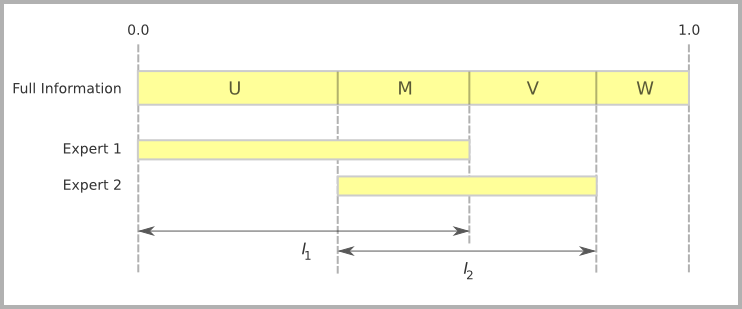
\includegraphics[width = \textwidth]{N=2} % requires the graphicx package
   \caption{Illustration of the partial information model with two experts.}
   \label{diagram2}
\end{figure}
Figure \ref{diagram2} illustrates this setup. In this diagram the Gaussian process has been partitioned into four parts based on the experts' information sets:
\begin{align*}
 U &= X_{I_1 / I_2}
& M &= X_{I_1 \cap I_2}\\
 V &= X_{I_2 / I_1}
& W &= X_{(I_1 \cup I_2)^c}
\end{align*}
Then,
\begin{align*}
X_{I_1} &= U + M\\
X_{I_2} &= M + V\\
X_S &= U+M+V+W,
\end{align*}
where $U, V, M, W$ are independent Gaussians with respective variances $\delta_1-\rho$, $\delta_2-\rho$, $\rho$, $1+\rho-\delta_1 - \delta_2$. The random variable $X_{I_j}$ can be interpreted as the information known by expert $E_j$. The joint distribution of $X_{S}$, $X_{I_1}$, and $X_{I_2}$ is a multivariate Gaussian distribution. That is,
\begin{align}
\left(\begin{matrix} X_S \\ X_{I_1}\\ X_{I_2} \end{matrix}\right) &\sim \mathcal{N}\left(
 \boldsymbol{0},  \left(\begin{matrix} 
1 & \delta_1 & \delta_2\\
\delta_1 & \delta_1 &\rho\\
\delta_2 & \rho & \delta_2
 \end{matrix}\right)\right) \label{twoExperts}
\end{align}
Given that $X_S$ has mean zero, the prior probability for the event is $\P(X_S > 0) = \P(A) = 0.5$. This can be easily adjusted to any probability $\tilde{p}$ by letting $A = \{ X_S > \Phi^{-1}(1-\tilde{p}) \}$. For instance, if the event to be predicted is one of a sequence of repeated events,  it may be reasonable to set $\tilde{p}$ to the empirical rate of occurrence of the already realized events. Given that this paper is not concerned with any particular event, the prior probability is  $\tilde{p} = 0.5$.  

\begin{figure}[htbp]
   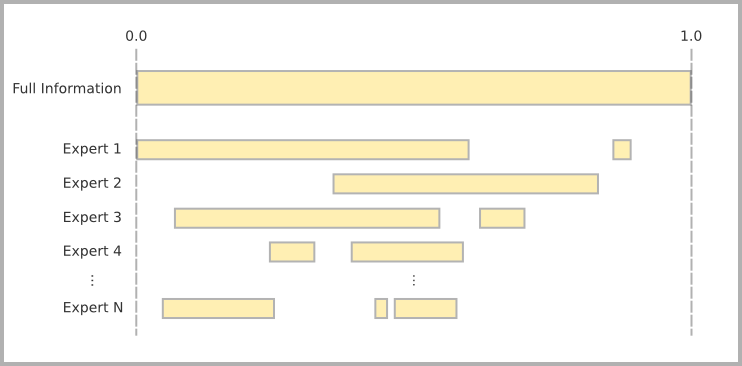
\includegraphics[width = \textwidth]{N=N} % requires the graphicx package
   \caption{Illustration of the partial information model with $N$ experts.}
   \label{diagramN}
\end{figure}



Consider now $N$ experts. Let $|I_j| = \delta_j$ be the amount of information known by expert $E_j$, and $|I_i \cap I_j| = \rho_{ij}$ be the information overlap between experts $E_i$ and $E_j$. Expression (\ref{twoExperts}) generalizes to the vector $(X_{S}, X_{I_1}, X_{I_2}, \dots, X_{I_N})$ as follows.
\begin{align}
\left(\begin{matrix} X_S \\ X_{I_1}\\ \vdots \\ X_{I_N} \end{matrix}\right) &\sim \mathcal{N}\left( \left(\begin{matrix} 
\mu_1 \\ \boldsymbol{\mu}_2
 \end{matrix}\right) =
 \boldsymbol{0}, \left(\begin{matrix} 
\Sigma_{11} & \Sigma_{12}\\
\Sigma_{21} & \Sigma_{22}\\
 \end{matrix}\right) 
 =
 \left(\begin{array}{c | c c cc }
1 & \delta_1 & \delta_2 & \dots & \delta_N  \\ \hline
\delta_1 & \delta_1 &\rho_{1,2} & \dots & \rho_{1,N}   \\ 
\delta_2 & \rho_{2,1} & \delta_2 & \dots & \rho_{2,N}  \\ 
\vdots & \vdots & \vdots & \ddots & \vdots  \\ 
\delta_N & \rho_{N,1} & \rho_{N,2} & \dots & \delta_N\\ 
 \end{array}\right)\right)  \label{NExperts}
\end{align}
This case is illustrated in Figure \ref{diagramN}. It is important to notice that $I_j$ does not have to be a contiguous segment of the unit interval. Instead, each expert can know any Borel measurable subset of the full information. Given that the information structure is described by the sub-matrix $\Sigma_{22}$, learning about the information among the $N$ experts is equivalent to estimating a covariance matrix under several restrictions. First, each element of $\Sigma_{22}$ must be in the unit interval, and no off-diagonal element can be larger than the corresponding diagonal element in the same row. Second, $\Sigma_{22}$ must be symmetric, non-singular, and coherent. The matrix $\Sigma_{22}$ is coherent if and only if its information structure can be described by a diagram such as the one given in Figure \ref{diagramN}. 


The next step is to link this model with the probability forecasts. If  $P_{I_j} = X_{I_j}/\sqrt{1-\delta_j}$ represents $E_j$'s probit-forecast, the corresponding probability forecast is given by
\begin{align}
p_j &= \P\left(A | \mathcal{F}_{I_j}\right) = \Phi\left( P_{I_j}\right) \label{Indiv}
\end{align}
Let $A_1, A_2, \dots$ be a infinite sequence of events, each defined similarly to $A$. If the $j$th expert's probability forecast for $A_i$ is given by (\ref{Indiv}), then the expert's forecasts align with the long-term frequency of the events. That is, when considering only those events for which $p_j$ takes on some preassigned value $p_j' \in [0, 1]$, the long term frequency of occurrence of those events is $p_j'$. Such an expert is deemed \textit{well-calibrated} (see, e.g., \cite{degroot1983comparison}). Given that several experiments have shown that experts are often poorly calibrated (see, e.g., \cite{cooke1991experts, shlyakhter1994quantifying}), assuming calibrated forecasts can be unrealistic. This could be remedied by  either including an additive error term in (\ref{Indiv}) such that the experts are on average calibrated, or by extending the total information by an amount unknown to the experts. Furthermore, if the experts make repeated forecasts for a sequence of events (e.g., whether it rains or not over a series of days), it may be possible to calibrate their forecasts (see, e.g., \citet{foster1998asymptotic, Brier}). All of these extensions, however, are considered beyond the scope of this paper and hence deferred to future work.

The marginal distribution of $p_j$ is
\begin{align*}
m(p_j | \delta_j) &= \sqrt{\frac{1-\delta_j}{\delta_j}} \exp \left\{ \Phi^{-1}(p_j)^2 \left(1-\frac{1}{2 \delta_j} \right) \right\} 
\end{align*}
This is uniform on $[0,1]$ if the $j$th expert knows half of the information, i.e. $\delta_j = 0.5$. If the expert knows less than half of the information, i.e. $\delta_j < 0.5$, the marginal distribution is unimodal at $0.5$ with the variance decreasing to 0 as $\delta_j \to 0$. Therefore an expert with no information always reports a ``non-informative" forecast of $0.5$. On other hand, if the expert knows more than half of the information, i.e. $\delta_j > 0.5$, the marginal  distribution is more heavily concentrated around extreme probabilities $0.0$ and $1.0$. More specifically, the marginal distribution becomes uniform over the set $\{0.0,1.0\}$ as $\delta_j \to 1$. Therefore an expert who knows all the information always reports the correct outcome. Figure \ref{marginals} illustrates the marginal distribution for $\delta_j$ equal to $0.3$, $0.5$, and $0.7$. 
%If these are considered inappropriate for the given context (e.g. symmetry is  unreasonable), it is possible to specify new marginals with a beta distribution and then apply a Gaussian copula to link the probability forecasts with the information sets (see, e.g.,  \cite{nelsen1999introduction} for an introduction on copulas). 

\begin{figure}[t]
\centering
	\hspace{0em}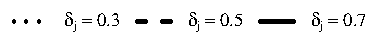
\includegraphics{LegendMarginal}

 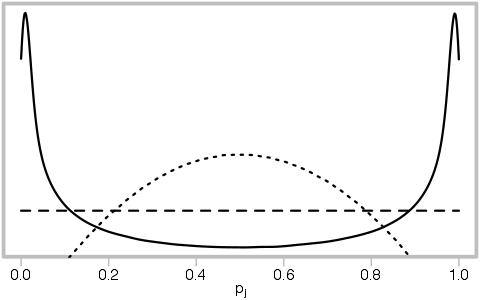
\includegraphics[width= 0.55\textwidth]{Marginals}
   \caption{The marginal distribution of $p_j$ under different levels of $\delta_j$. The more the expert knows, i.e. the higher $\delta_j$ is, the more the probability forecasts are concentrated around the extreme points 0.0 and 1.0.}
\label{marginals}
\end{figure}


\section{Probability Extremizing}
\label{extremizing}
%\textcolor{red}{Write about extremizing wrt average probability}
The best in-principle forecast given the knowledge of $N$ experts is $\P(X_{S} > 0 |  \mathcal{F}')$, where $\mathcal{F}' = \mathcal{F}_1 \cup \dots \cup \mathcal{F}_N$. In this paper such an aggregate forecast is called the \textit{crowd belief}. Even though in practice knowledge of $\mathcal{F}'$ is almost always unattainable due to company confidentiality or the experts' inability to specify the knowledge that ultimately leads to their opinions (\cite{dawid1995coherent}), in theory the crowd belief can be obtained by introducing an ``oracle" expert whose information set is $I' = I_1 \cup \dots \cup I_N$. Therefore the oracle  knows everything that the group of experts knows. The oracle can be added to the multivariate Gaussian distribution (\ref{NExperts}) as follows.
\begin{align}
\left(\begin{matrix} X_S \\ X_{I'} \\ X_{I_1}\\ \vdots \\ X_{I_N} \end{matrix}\right) &\sim \mathcal{N}\left( 
 \boldsymbol{0}, \left(\begin{matrix} 
\Sigma_{11}' & \Sigma_{12}'\\
\Sigma_{21}' & \Sigma_{22}\\
 \end{matrix}\right) 
 =
 \left(\begin{array}{c c| c c cc }
1 & \delta' & \delta_1 & \delta_2 & \dots & \delta_N  \\ 
\delta' & \delta' & \delta_1 & \delta_2 & \dots & \delta_N  \\ \hline
\delta_1& \delta_1 & \delta_1 &\rho_{1,2} & \dots & \rho_{1,N}   \\ 
\delta_2 & \delta_2 &\rho_{2,1} & \delta_2 & \dots & \rho_{2,N}  \\ 
\vdots &\vdots & \vdots & \vdots & \ddots & \vdots  \\ 
\delta_N &\delta_N & \rho_{N,1} & \rho_{N,2} & \dots & \delta_N\\ 
 \end{array}\right)\right),  \label{NExpertsOracle}
\end{align}
where  $X_{I'}$  is the information known by the oracle and $\delta' = |I'|$ is the amount of this information. 

Similarly to the individual experts, the oracle's probability forecast, i.e. the crowd belief, is given by 
 \begin{align}
p^{crowd}_N = \P(X_S > 0 |  \mathcal{F}') &= \Phi\left( \frac{X_{I'}}{\sqrt{1-\delta'}} \right)
\end{align}
This forecast is calibrated and efficiently utilizes all the information among the experts. Therefore it provides the ``gold standard'' for analyzing probability extremizing, which is understood as an increase in the strength of the belief indicated by the probability forecast. More specifically, a probability $p$ is extremized by another probability $p'$ if and only if $p'$ is closer to $0$ when $p \leq 0.5$ and closer to $1$ when $p \geq 0.5$. This can be expressed more succinctly in terms of probits as follows: if $P = \Phi^{-1}(p)$, $P' = \Phi^{-1}(p')$, and $\alpha$ is a real-valued constant such that $\alpha P = P'$, then $p'$ extremizes $p$ when $\alpha > 1$. Therefore $\alpha$ is a univariate quantity that represents the multiplicative amount of extremizing that $p'$ performs for $p$. Letting $p= p_{N}^{ave\ prb}$ and $p' = p_N^{crowd}$ gives
%\footnote{Even though this paper focuses on extremizing of $p_N^{ave\ prb}$, the discussion can be easily adapted to $p_N^{ave\ log}$ by recalling the following approximation (see, e.g., \cite{train2009discrete}).
%\begin{align*}
% \log\left\{\frac{p_j}{1-p_j}\right\} &\approx \Phi^{-1}(p_j)/\sqrt{\frac{\pi}{8}}
%\end{align*}
%Therefore the amount of extremizing of $p_N^{ave\ log}$ is approximately $\alpha \sqrt{\frac{\pi}{8}}$.}
\begin{align}
\alpha  = \frac{P_{I'}}{\frac{1}{N}\sum_{j=1}^N P_{I_j}}\label{alpha}
\end{align}
%The partial information aggregate $p_N^{info}$ extremizes $p_N^{ave\ prb}$ when $\alpha$ is greater than one. On the other hand, when $\alpha$ is less than one, $p_N^{info}$ reverse-extremizes $p_N^{ave\ prb}$.
%If $\delta_j = \delta'$ for all $j = 1, \dots, N$, then average probit coincides with the oracle's probit and $\alpha$ is always equal to $1.0$. If, on the other hand, $\delta_j \neq \delta'$ for some $j = 1, \dots, N$, the amount of extremizing $\alpha$ 
%If $\delta_j \neq \delta'$  for some $j = 1, \dots, N$ and $\delta' \neq 1$, then $\alpha$ 
This is a random quantity that spans the entire real line. That is, it is possible to find a set of probability forecasts and a distribution of information for any possible value of $\alpha \in \mathbb{R}$. Therefore extremizing is not guaranteed to always improve the probit opinion pool. To understand when extremizing is likely to be beneficial, it is necessary to derive the probability distribution of $\alpha$. First, given that 
\begin{align*}
P_{I'} &\sim \mathcal{N}\left(0, \sigma^2_{1} = \frac{\delta'}{1-\delta'} \right)\\
\frac{1}{N}\sum_{j=1}^N P_{I_j} &\sim \mathcal{N}\left\{0, \sigma^2_{2} =\frac{1}{N^2} \left( \sum_{j=1}^N \frac{\delta_j}{1-\delta_j} + 2 \sum_{i,j: i<j} \frac{\rho_{ij}}{\sqrt{(1-\delta_j)(1-\delta_i)}}\right) \right\},
\end{align*}
the amount of extremizing $\alpha$ is a ratio of two correlated Gaussian random variables. The Pearson product-moment correlation coefficient for them is
\begin{align*}
%corr\left(P_{I'}, \frac{1}{N}\sum_{j=1}^N P_{I_j} \right) &= \frac{\frac{1}{N} \sum_{j=1}^N \frac{\delta_j}{\sqrt{(1-\delta')(1-\delta_j)}}}{\sqrt{\frac{\delta'}{1-\delta'} \frac{1}{N^2} \left( \sum_{j=1}^N \frac{\delta_j}{1-\delta_j} + 2 \sum_{i,j: i<j} \frac{\rho_{ij}}{\sqrt{(1-\delta_j)(1-\delta_i)}}\right)}}\\
\kappa  &= \frac{ \sum_{j=1}^N \frac{\delta_j}{\sqrt{1-\delta_j}}}{\sqrt{\delta'  \left( \sum_{j=1}^N \frac{\delta_j}{1-\delta_j} + 2 \sum_{i,j: i<j} \frac{\rho_{ij}}{\sqrt{(1-\delta_j)(1-\delta_i)}}\right)}}
\end{align*}
The amount of extremizing $\alpha$ then follows a Cauchy distribution as long as $\sigma_1 \neq 1$, $\sigma_2 \neq 1$, or $\kappa \pm 1$ (see, e.g., \cite{cedilnik2004distribution} for this well-known result). These conditions are very mild under the partial information model. For instance, if no expert knows as much as the oracle, the conditions are satisfied. Consequently, the probability density function of $\alpha$ is
\begin{align}
f(\alpha | x_0, \gamma) &= \frac{1}{\pi} \frac{\gamma}{(\alpha-x_0)^2+\gamma^2}, \label{Cauchy}
\end{align}
where 
\begin{align*}
x_0 = \kappa \frac{\sigma_1}{\sigma_2} && \gamma &= \frac{\sigma_1}{\sigma_2} \sqrt{1-\kappa^2}
\end{align*}
The parameter $x_0$ represents the location (the median and mode) and $\gamma$ specifies the scale (half the interquartile range) of the Cauchy distribution. It is possible to show that $x_0 \geq 1$. This leads to the following theorem whose proof is deferred to Appendix A.

\begin{theorem}
\label{positiveProbThm}
%Under the partial information model, the probability $\P(\alpha \geq 1 | \Sigma_{22}) \in (0.5,1]$.
 If $\delta_j \neq \delta'$ for some $j = 1, \dots, N$, then the probability that the probit opinion pool requires extremizing is $\P(\alpha > 1 | \Sigma_{22}) \in (0.5,1]$, where the bounds are sharp.
\end{theorem}
\noindent
This theorem shows that, on any non-trivial problem, extremizing is more likely to be improve the probit opinion pool than to degrade it. This can partially explain why extremizing aggregators perform well on large sets of real-world prediction problems.  To understand how the probability $\P(\alpha > 1 | \Sigma_{22})$  changes across different information structures,  
%Given that (\ref{Cauchy}) depends on $2+N(N+1)/2$ parameters,
 it is helpful, if not necessary, to make simplifying assumptions. A natural choice is to consider all experts exchangeable and develop intuition at a higher level. This is done in the next subsection that analyzes extremizing under compound symmetric information. 




\subsection{Extremizing under Compound Symmetric Information}
\label{compound}

This section assumes that the experts' information sets have the same size and that the amount of overlap between any two information sets is constant, i.e.  $|I_{1}| =  \dots = |I_{N}|$ and $|I_{i} \cap I_{j}| = |I_{h} \cap I_{k}|$ for all $i \neq j$ and $h \neq k$. In other words, each expert knows and shares the same amount of information with every other expert. The corresponding information structure $\Sigma_{22}$ is compound symmetric. That is,
% $\rho \in [\max \{(N-T)/(T(N-1)), 0\},1] = A_\rho$. 
\begin{align*}
\left(\begin{matrix} X_{S} \\ X_{I'}\\ X_{I_1}\\ \vdots \\ X_{I_N} \end{matrix}\right) &\sim \mathcal{N}\left( 
 \boldsymbol{0}, \left(\begin{matrix} 
\Sigma_{11}' & \Sigma_{12}'\\
\Sigma_{21}' & \Sigma_{22}\\
 \end{matrix}\right) 
 =
 \left(\begin{array}{cc|cccc}
1 & \delta'& \delta & \delta & \dots & \delta  \\ 
\delta' & \delta' & \delta & \delta & \dots & \delta  \\ \hline
\delta & \delta &\delta & \lambda\delta & \dots & \lambda\delta   \\ 
\delta& \delta & \lambda\delta & \delta & \dots & \lambda\delta  \\ 
\vdots &\vdots & \vdots & \vdots & \ddots & \vdots  \\ 
\delta &\delta & \lambda\delta & \lambda\delta & \dots & \delta\\ 
 \end{array}\right)\right)
\end{align*}
%where the super-script $(cs)$ emphasizes that this information structure is compound symmetric and hence different from the fully general structure described in (\ref{NExperts}). Only the top-left block of the covariance matrix is the same as in (\ref{NExperts}). 
The amount of information known by each expert is denoted with $\delta \in [0,1]$. The value of $\lambda$ is the proportion of the known information that is shared between any two experts.  This minor change of parametrization was made for the sake of simplifying some of the following expressions. To ensure that $\Sigma_{22}$ is coherent, a domain restriction must be placed on $\lambda$. 
%The upper bound for $\lambda$ is given by $1$ because 
First, given that under any combination of $\delta$ and $N$, it is possible that all experts know the exact same information. the value of $\lambda$ is upper bounded by $1$. Second, observe that information overlap is unavoidable when $\delta > 1/N$. The minimum sharing occurs when all information is either shared or private. In other words, if $\delta > 1/N$ and $I_{i} \cap I_j = I$ with $|I| =  \lambda \delta$ for all $i \neq j$, the value of $\lambda$ is minimized when $\lambda\delta + N(\delta - \delta\lambda) = 1$. Therefore the lower bound for $\lambda$ is $\max \left\{ \frac{N-\delta^{-1}}{N-1}, 0\right\}$, and $\Sigma_{22}$ is coherent if and only if
\begin{align}
\delta \in [0,1] &&  \lambda &\in \left[  \max \left\{ \frac{N-\delta^{-1}}{N-1}, 0\right\}, 1 \right), \label{rhoDomain}
\end{align}
where the open upper bound on $\lambda$ ensures a non-singular $\Sigma_{22}$. 

%The quantity  $\lambda\delta + N(\delta - \delta\lambda)$ also describes the maximum information coverage of the $N$ experts, i.e. $\max | I_1 \cup I_2 \cup \dots \cup I_N| = \lambda\delta + N(\delta - \delta\lambda)$. 

%To make this more explicit, observe that the Jacobian for the map $\boldsymbol{P} \to \Phi\left(\boldsymbol{P}\right) = (\Phi(p_1), \Phi(p_2), \dots, \Phi(p_N))$ is
%\begin{eqnarray*}
%J(\boldsymbol{P}) &=& (2\pi)^{-N/2} \exp \left( - \frac{\boldsymbol{P}' \boldsymbol{P}}{2}   \right) 
%\end{eqnarray*}
%%
%%$\boldsymbol{P} \sim \mathcal{N}_N\left(\boldsymbol{0}, \Sigma_{22} (1-\delta)^{-1}\right)$ and that
%Represent a $N\times N$ matrix of ones with $J_{N \times N}$. If $h(\boldsymbol{P})$ denotes the multivariate Gaussian density of $\boldsymbol{P} \sim \mathcal{N}_N\left(\boldsymbol{0}, \Sigma_{22} (1-\delta)^{-1}\right)$,
%%by the Inverse Function Theorem 
%the density for  $\boldsymbol{p} = (p_1, p_2, \dots, p_N)$ becomes
%\begin{eqnarray*}
% f\left(\boldsymbol{p} | \delta, \lambda \right) &=& h(\boldsymbol{P}) J(\boldsymbol{P})^{-1} \bigg|_{\boldsymbol{P} = \Phi^{-1}(\boldsymbol{p})}\\
%%&=& \frac{(1-\delta)^{N/2}}{\sqrt{ |\Sigma_{22}|}} \exp\left( -\frac{1}{2} \boldsymbol{P}' (1-\delta)\Sigma_{22}^{-1} \boldsymbol{P} + \frac{\boldsymbol{P}' \boldsymbol{P}}{2}   \right)\\
%&=& \frac{(1-\delta)^{N/2}}{\sqrt{ \left|\Sigma_{22}\right|}} \exp\left[ -\frac{1}{2} \Phi^{-1}(\boldsymbol{p})' \left\{ (1-\delta) \Sigma_{22}^{-1} - I_N \right\} \Phi^{-1}(\boldsymbol{p})  \right],
%\end{eqnarray*}
%%where $\Phi^{-1}(\boldsymbol{p}) =  (\Phi^{-1}(p_1), \Phi^{-1}(p_2), \dots, \Phi^{-1}(p_N))$. 
%%Given that $\Sigma_{22}$ can be written in the form  $\Sigma_{22} = I_N (\delta-\lambda\delta) + J_{N \times N} \lambda\delta$
%where
%%The determinant and inverse of $\Sigma_{22}$ are
%\begin{align}
%\left| \Sigma_{22}\right| &= (\delta(1- \lambda))^N \left(1+\frac{N \lambda}{1 - \lambda} \right) \nonumber\\
%\Sigma_{22}^{-1} &= I_N \left(\frac{1}{\delta-\lambda\delta} \right) - J_{N \times N} \frac{\lambda}{(1-\lambda)\delta\{1+(N-1) \lambda\}} \label{inverse}
%\end{align}
%See \cite{rao2009linear} and the supplementary material of \cite{dobbin2005sample} for the derivations of the determinant and inverse of $\Sigma_{22}$, respectively. The maximum likelihood estimates of $\delta$ and $\lambda$ are then obtained from
%\begin{align*}
%\left(\hat{\delta}, \hat{\lambda}\right) =& \argmax_{\lambda, \delta} \log  f\left(\boldsymbol{p}| \delta, \lambda \right),\\
%& \text{s.t. } \nonumber \delta \in [0,1] \text{ and } \lambda \in \left[  \max \left\{ \frac{N-\delta^{-1}}{N-1}, 0\right\}, 1 \right)
%\end{align*}
%Unfortunately, this  cannot be solved analytically. A simple grid-search, however, can be used to find the estimates very efficiently. 

%\begin{align*}
%(\hat{\delta}, \hat{\lambda}) &= \argmax_{\lambda, \delta}  - \frac{N}{2} \log (\delta - \lambda\delta) - \frac{1}{2} \log \left(1+\frac{N \delta \lambda}{\delta - \delta\lambda} \right) -\frac{1}{2} \boldsymbol{X}' \left( I_N \left(\frac{1}{\delta-\lambda\delta} \right) - J_{N \times N} \frac{\lambda}{(1-\lambda)\delta(1+(N-1) \lambda)}  \right) \boldsymbol{X}
%\end{align*}




%Recall that if $X_{I_j} \sim \mathcal{N}(0,1)$, then $\Phi(X_{I_j})$ is uniform on $[0,1]$. Therefore, if $\delta_j = 1$, the marginal distribution of $p_j = \Phi(X_{I_j})$ is uniform on $[0,1]$. If this does not hold empirically, it is a sign that the model cannot be correct on the micro-level. If $X_{I_j}$ appears more (respectively less) concentrated about $0.5$, then the model can be adjusted by changing $\delta_{j}$ to a smaller fraction. 


%Assuming no further prior information on overlap structure, the expected amount of information held by the group is WHAT IS THIS?

%The aggregator under the compound symmetric information structure is derived by first applying (\ref{inverse}) to the general formulas (\ref{condMu}) and (\ref{condSigma}). The resulting conditional mean and variance are 
%By the conditional multivariate normal results, we have that 
%\begin{align*}
%\bar{\mu} &= \mu_1 + \Sigma_{12} \Sigma_{22}^{-1} (\boldsymbol{X} - \boldsymbol{\mu}_2)\\
% &= \Sigma_{12} \Sigma_{22}^{-1} \boldsymbol{X} \\
% \\
% \bar{\Sigma}&= \Sigma_{11} - \Sigma_{12} \Sigma_{22}^{-1} \Sigma_{21}\\
%&=1 - \Sigma_{12} \Sigma_{22}^{-1} \Sigma_{21}
%\end{align*}
%
%%(see \url{http://linus.nci.nih.gov/techreport/DobbinSimonAppendix.pdf} for this). 
%Hence the off-diagonals of $\Sigma_{22}^{-1}$ are 
%\begin{align*}
%\frac{\lambda\delta}{(\lambda\delta-\delta)((N-1)\lambda\delta +\delta)}
%\end{align*}
%and the diagonals are
%\begin{align*}
%\frac{(2-N)\lambda\delta -\delta}{(\lambda\delta-\delta)((N-1)\lambda\delta +\delta)}
%\end{align*}
%The conditional mean can be derived as
%\begin{align*}
%\Sigma_{22}^{-1} &= \frac{1}{(\lambda\delta-\delta)((N-1)\lambda\delta +\delta)}
% \left(\begin{matrix} 
%(2-N)\lambda\delta -\delta & \lambda\delta & \dots & \lambda\delta \\ 
%\lambda\delta & (2-N)\lambda\delta -\delta & \dots & \lambda\delta \\ 
%\vdots & \vdots &  \ddots & \vdots \\ 
%\lambda\delta & \lambda\delta & \dots & (2-N)\lambda\delta -\delta  \\ 
% \end{matrix}\right)\\
% \Sigma_{12} \Sigma_{22}^{-1} &= \frac{\delta}{(\lambda\delta-\delta)((N-1)\lambda\delta +\delta)} \left( \begin{matrix} \lambda\delta -\delta &  \dots & \lambda\delta -\delta \end{matrix} \right)\\
% \Sigma_{12} \Sigma_{22}^{-1} \boldsymbol{X} &= \frac{\delta}{(\lambda\delta-\delta)((N-1)\lambda\delta +\delta)} (\lambda\delta -\delta) \sum_{j=1}^N X_j \\
%&= \frac{\delta(\lambda\delta -\delta)}{(\lambda\delta-\delta)((N-1)\lambda\delta +\delta)}  \sum_{j=1}^N X_j \\
%&= \frac{\delta}{(N-1)\lambda\delta +\delta}  \sum_{j=1}^N X_j \\
%\begin{align*}
%\bar{\mu} = \frac{1}{(N-1)\lambda +1}  \sum_{j=1}^N X_j 
% \bar{\Sigma} &= 1 -  \Sigma_{12} \Sigma_{22}^{-1}\Sigma_{21} \\
% &= 1  - \frac{\delta^2}{(\lambda\delta-\delta)((N-1)\lambda\delta +\delta)} N(\lambda\delta -\delta)\\
% &= 1  - \frac{\delta^2N}{(N-1)\lambda\delta +\delta} \\
%&&  \bar{\Sigma} = 1  - \frac{\delta N}{(N-1)\lambda +1} 
%\end{align*}
Plugging these simplifications in (\ref{alpha}) gives 
\begin{align}
\alpha &= \frac{X_{I'}}{\frac{1}{N}\sum_{j=1}^N X_{I_j}} \sqrt{\frac{1-\delta}{1-\delta'}} \label{CompoundAlpha}
\end{align}
%If $\delta$ is much smaller than $\delta'$,  the experts must have low information overlap $\delta$. In other words, the experts present high information diversity. This is quantified by the term $\sqrt{(1-\delta)/(1-\delta')} \in [1, \infty)$ that is small (or large) when the experts possess low (or high) information diversity. Therefore, assuming that the 
%Observe that $\alpha = 1$ when $\lambda = 1$, i.e. when all the experts know the same information. Consequently, the group of expert is equivalent to a single expert, and the probit opinion pool coincides with the oracle aggregate. Therefore no extremizing is required. 
%The amount of this extremizing increases in $\delta$ and decreases in $\lambda$, or more succinctly stated, increases in the total amount of information among the expert $\delta'$. 
This follows a $\text{Cauchy}(x_0, \gamma)$ with
\begin{align*}
x_0 &= \frac{N}{1+(N-1)\lambda}  \sqrt{\frac{1-\delta}{1-\delta'}}\\
 \gamma &=  \sqrt{\frac{N(\delta' + \delta' \lambda (N-1) - \delta N)}{\delta (\lambda (N-1) + 1)^2}}\sqrt{\frac{1-\delta}{1-\delta'}}
\end{align*}
The total amount of information among the experts $\delta'$ is uniquely determined by $\delta$ and $\rho$ when the group involves only two experts. More specifically, $\delta' = 2\delta - \delta\lambda$ when $N=2$. Therefore, by assuming only two experts, both $x_0$ and $\gamma$ can be analyzed graphically under different information structures. Figure \ref{LevelplotsOracle} shows $\log(x_0)$, $\gamma$, and $\P(\alpha > 1 | \Sigma_{22})$ under all plausible combinations of $\delta$ and $\rho$. High values have been censored to keep the scale manageable. 

\begin{figure}[t]
%\centering
%%\hspace*{2em}  $\log(\alpha)$
%\hspace*{1.2em} 	\includegraphics[width=0.973\textwidth, height = 3em]{colorkey} % requires the graphicx package
\hspace{-1.2em}
        \centering
        \begin{subfigure}[b]{0.33\textwidth}
                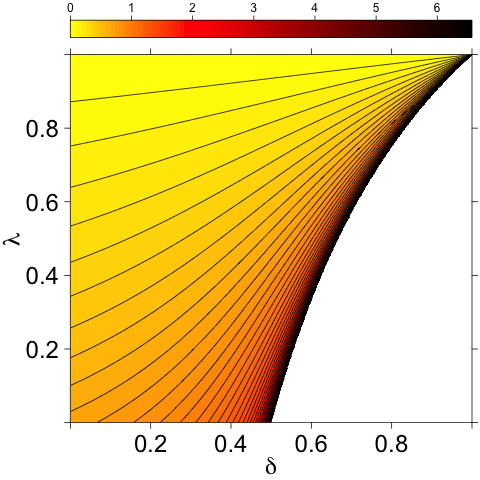
\includegraphics[width=1.07\textwidth, height = \textwidth]{ExtremeX0}
\caption{$\log(x_0)$}	
\label{xOracle}
        \end{subfigure}%
\hspace{0.6em}
        \begin{subfigure}[b]{0.33\textwidth}
                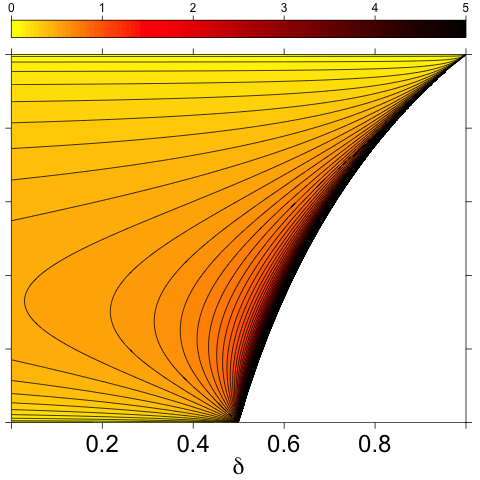
\includegraphics[width= 0.95\textwidth, height = \textwidth]{ExtremeGamma}
\caption{$\gamma$}
\label{gammaOracle}
        \end{subfigure}
\hspace{-1.3em}
        \begin{subfigure}[b]{0.33\textwidth}
                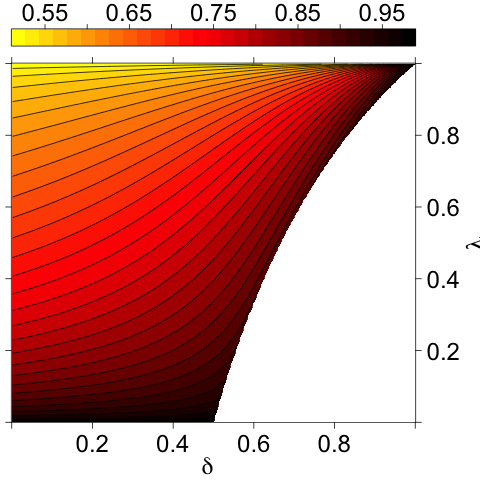
\includegraphics[width=1.07\textwidth, height = \textwidth]{Probs}
\caption{$\P(\alpha > 1 | \Sigma_{22})$}
\label{probOracle}
        \end{subfigure}

        \caption{ The amount of extremizing follows a Cauchy$(x_0, \gamma)$, where $x_0$ is a location parameter and $\gamma$ is a scale parameter. This figure considers only $N = 2$ experts and shows $\log(x_0)$, $\gamma$, and $\P(\alpha > 1 | \Sigma_{22})$ under all plausible combinations of $\delta$ and $\lambda$.}
        \label{LevelplotsOracle}
\end{figure}
 

According to Figure \ref{LevelplotsOracle} extremizing is required more often when $\delta$ is high and $\lambda$ is low. Given that $\delta'$ increases in $\delta$ but decreases in $\lambda$, the amount of extremizing can be expected to increase in the total amount of information among the experts $\delta'$. This, however, does not provide a full explanation of extremizing. Information diversity is also an important yet separate determinant of extremizing. To see this, observe that fixing $\delta'$ to some constant defines a curve $\lambda = 2 - \delta'/\delta$ on the plots in Figure \ref{LevelplotsOracle}. For instance, letting $\delta' = 1$ gives the boundary curve on the right side of each plot. This curve then shifts inwards and rotates slightly counterclockwise as $\delta'$ decreases. At the top end of each curve all experts know and share the total information, i.e. $\delta = \delta'$ and $\lambda = 1.0$.  At the bottom end, on the other hand, the experts partition the total information, i.e. $\delta = \delta'/2$, and share nothing, i.e. $\lambda = 0.0$. Therefore moving down along the curve increases information diversity among the experts. Given that at the same time the expected amount of extremizing increases, information diversity can be considered as an important determinant of extremizing together with the group's total information. 

This relationship can be understood in broader terms as follows. Recall that the experts form their individual forecasts independently based on their own information. Given that this personal information cannot be larger than the group's total information, the expert's forecast is often less confident, i.e. closer to $0.5$, than the crowd belief. Unfortunately, any average of the individual forecasts cannot be more confident than the most confident expert in the group. Therefore it cannot extend beyond convex hull of the individual forecasts even when this is suggested by the group's total information. The crowd belief, on the other hand, is based on more information than any of the individual forecasts, and as a result, is likely to be more confident than any of them. The gap between the average aggregate and the crowd belief widens as the group's total information increases (the crowd belief becomes more confident) and the average amount information of a single expert decreases (the convex hull becomes more concentrated around $0.5$ and the average aggregate becomes less confident). These two changes can happen simultaneously only if the information diversity among the experts increases. 


In Figure \ref{xOracle} the location parameter $x_0 \geq 1$ and, consequently, $\P(\alpha > 1 | \Sigma_{22}) \in (0.5, 1.0]$. This follows from Theorem \ref{positiveProbThm}. As $\lambda \uparrow 1.0$, the location $x_0 \uparrow 1.0$ and scale $\gamma \downarrow 0.0$, which represents a point mass at $\alpha = 1.0$.  In this case, all information is public, and the group of experts is as good as a single expert. Therefore, given that the forecast of a group with only one expert coincides with the crowd belief, $\lambda \uparrow 1.0$ always implies $\alpha \downarrow 1.0$ regardless of the value of $\delta$. From the top of Figure (\ref{xOracle}) the location $x_0$ increases indefinitely towards the boarder line defined by $\delta' = 2\delta - \delta\lambda = 1$. At this point the oracle knows everything and the crowd belief is always equal to the true outcome of the target event. Based on Figure \ref{probOracle}, the probit opinion pool is more likely to agree with the crowd belief at points closer to the end points of the boarder line, namely, when $(\delta, \lambda) = (0.5, 0.0)$ or  $(\delta, \lambda) = (1.0, 1.0)$. At the former point, experts' information sets form a partition of the full information. Therefore the experts know all the information. Such a group of experts can re-construct $X_S$ by simply adding up their information, and aggregation becomes deterministic voting: if the sum of the probit-forecasts is above $0.0$, the event $A$ materializes; else it does not. A similar observation has been made under the interpreted forecasts (\cite{hong2009interpreted}). At the latter point, the outcome of the target event is public information and the experts can deterministically report the correct outcome. In between these two points, however, there is a chance that the probit opinion pool disagrees with the crowd belief on the more likely outcome of the target event. The correction requires a large but negative value of $\alpha$. Consequently, the scale $\gamma$ increases and $\P(\alpha > 1 | \Sigma_{22})$ decreases slightly. 




%each expert is very knowledgeable, i.e. high $\delta$, and the group of experts is diverse, i.e. low $\lambda$. Therefore the amount to extremizing is determined by the total amount of information among the experts $\delta'$ and the 


%Given that $\delta'$ increases monotonically in $N$, the location parameter $x_0$ also increases in $N$ (holding both $\delta$ and $\lambda$ fixed). 

%In practice, however, the experts' information structure is likely to be well inside the interior of the set of plausible values of $\delta$ and $\lambda$.  Over most parts of the interior, the probability $\P(\alpha \geq 1 | \Sigma_{22})$ is considerably high. For instance, inside the rectangle defined by $\delta \in [0.2, 0.4]$ and $\lambda \in [0.3, 0.7]$ the probability $\P(\alpha \geq 1 | \Sigma_{22})$ ranges from 


The amount of extremizing is positive only if the probit opinion pool and the crowd belief are on the same side of $0.5$. The probability of this happening increases in $\P(\alpha > 1 | \Sigma_{22})$, which according to Figure \ref{probOracle} decreases in $\lambda$. Given that increasing $\lambda$ results in more similar probability forecasts, the value of $\lambda$ is inversely proportional to the variance of the forecasts. Therefore,  under the partial information model, higher variance can be considered helpful because it increases the chances of the probit opinion pool being on the same side $0.5$ with the crowd belief. Contrast this with the classical measurement error model where increased variance is typically considered harmful. This reversal of the effect is an important property of the interpreted forecasts (\cite{hong2009interpreted}). 

%The next section introduces an aggregator that does not depend on the knowledge of $\delta'$. Therefore it can be potentially applied in practice. The corresponding amount of extremizing under compound symmetric information depends only on the information structure $\Sigma_{22}$ -- not on $\boldsymbol{X}$. Therefore it is non-random and can be conveniently analyzed under any combination of $\delta$, $\lambda$, and $N$. The results present patterns that are very similar to the ones given in Figure \ref{LevelplotsOracle}.


%%where 
%%\begin{align*}
%%\gamma &= \frac{N}{(N-1)\lambda +1}\\
%%&= \left( \frac{1}{(N-1)\lambda +1} \right) N\\
%%\end{align*}
%%WHAT IS GAMMA? Given that 
%%\begin{align*}
%%\gamma \delta &\leq 1\\
%%% \frac{N \delta}{(N-1)\lambda +1}  &\leq& 1\\
%% \frac{N\delta - 1}{N-1}  &\leq \lambda,
%%\end{align*}
%The domain restriction (\ref{rhoDomain}) ensures that the term under the square-root in (\ref{CompoundAlpha}) is always non-negative.  
%%Given that the square-root is not defined for negative values,  it must be required that
%%\begin{align}
%%1- \frac{N\delta}{(N-1)\lambda +1}  &\geq 0 &\Leftrightarrow&& \lambda \geq \frac{N\delta - 1}{N-1} \label{rhoDomain2}
%%\end{align}
%%Compare this with former domain restriction (\ref{rhoDomain}) and observe that both $N\delta - 1$ and $N - \delta^{-1}$ are negative when $\delta < 1/N$. Given that $N\delta - 1 > N - \delta^{-1}$ only when $\delta < 1/N$, the latter restriction (\ref{rhoDomain2}) is redundant and can be ignored. 
%Given that (\ref{CompoundAlpha}) is increasing in $N$ and $\delta$ but decreasing in $\lambda$, the amount of extremizing can be considered increasing in the total amount of information among the experts. Recall from earlier discussion that the compound symmetric information structure invalidates the possibility of a dominant expert. As (\ref{CompoundAlpha}) does not depend on $\boldsymbol{X}$, the amount of extremizing cannot be driven by highly influential information either. Therefore the amount of extremizing is unaffected by both causes of reverse-extremizing. Consequently, the aggregator (\ref{CompoundAggre}) always extremizes $p_N^{ave\ prb}$.   This is stated more formally in the following Theorem along with the fact that the aggregator (\ref{CompoundAggre}) can leave the convex hull of the individual probabilities. The proof is deferred to Appendix A. 
%
%\begin{theorem}
%\label{positiveThm}
%Under the compound symmetric information structure, (a) the amount of extremizing $\alpha$ is always greater or equal to 1, and (b) the aggregator can leave the convex hull of the probability forecasts. 
%\end{theorem}
%
%The second part of Theorem \ref{positiveThm} states that aggregator (\ref{CompoundAggre}) is suitable for interpreted probability forecasts. Furthermore, given that in practice the values of $\delta$ and $\lambda$ can be estimated directly from the probability forecasts via the maximum likelihood method (see Appendix A for the details), aggregator (\ref{CompoundAggre}) can be used for combining interpreted probability forecasts of a one-time event. To the best of our knowledge, this is the first model-based aggregator that has been developed for such circumstances.
%\textcolor{red}{This is a first order approximation -- similar in level to the classical measurement error aggregators. Thereefore somehow it seems that the extremizing results are more relevant}
%




\section{Probability Aggregation}
Assuming knowledge of the union of the experts' information sets is hardly reasonable in practice. Therefore the best aggregate probability that can be realistically hoped for is  $\P(X_{S} > 0 | p_1, \dots, p_N)$.  This can be constructed under the partial information model by first deriving the conditional distribution of $X_S$ given $\boldsymbol{X}$. That is, if $\boldsymbol{X} = (X_{I_1}, X_{I_2},  \dots, X_{I_N})'$ is a column vector of length $N$ and $\Sigma_{22}$ is a coherent overlap structure such that $\Sigma_{22}^{-1}$ exists, then 
\begin{align*}
X_{S} | \boldsymbol{X} \sim \mathcal{N}(\bar{\mu}, \bar{\Sigma}), 
\end{align*}
where
\begin{align}
\bar{\mu} &= \mu_1 + \Sigma_{12} \Sigma_{22}^{-1} (\boldsymbol{X} - \boldsymbol{\mu}_2) =  \Sigma_{12} \Sigma_{22}^{-1} \boldsymbol{X} \label{condMu}\\
 \bar{\Sigma}&= \Sigma_{11} - \Sigma_{12} \Sigma_{22}^{-1} \Sigma_{21} =1 - \Sigma_{12} \Sigma_{22}^{-1} \Sigma_{21}  \label{condSigma}
\end{align}
These expressions can be found directly from the formulas of the conditional multivariate Gaussian distribution (see, e.g., Result 5.2.10 on p. 156 in \cite{ravishanker2001first}). This then leads to a probability aggregator that depends on $\Sigma_{22}$. More specifically, the partial information aggregator is
\begin{align}
p_N^{info} = \P\left(A  | \boldsymbol{X}\right)  = \P\left(X_{S} > 0 | \boldsymbol{X}\right) &= \Phi\left( \frac{\Sigma_{12} \Sigma_{22}^{-1} \boldsymbol{X}}{\sqrt{1 - \Sigma_{12} \Sigma_{22}^{-1} \Sigma_{21}}}\right) \label{GeneralAggregator}
%&= \Phi\left( \frac{\boldsymbol{1}_{N}'  \Sigma_{22}^{-1} \Phi^{-1}(\boldsymbol{p})}{\sqrt{1 - \boldsymbol{1}_{N}' \Sigma_{22}^{-1} \boldsymbol{1}_{N}}}\right)
\end{align}
Furthermore, if $\boldsymbol{1}_N$ is a column vector of ones and $\boldsymbol{P} = (P_{I_1}, P_{I_2}, \dots, P_{I_N})'$, then the amount of extremizing that $p_N^{info}$ performs for $p_{N}^{ave\ prb}$ is
% such that the average probit-forecast is $\bar{P} = \boldsymbol{1}_N' \boldsymbol{P} /N$. 
\begin{align}
%\alpha \bar{P}&=  \frac{\Sigma_{12} \Sigma_{22}^{-1} \boldsymbol{X}}{\sqrt{1 - \Sigma_{12} \Sigma_{22}^{-1} \Sigma_{21}}}  &\Leftrightarrow&& 
\alpha  &= \frac{N \Sigma_{12} \Sigma_{22}^{-1} \boldsymbol{X}}{\left(\boldsymbol{1}_N' \boldsymbol{P} \right) \sqrt{1 - \Sigma_{12} \Sigma_{22}^{-1} \Sigma_{21}}} \label{alpha}
\end{align}
Given that accurate estimation of the fully general information structure $\Sigma_{22}$ based on the probability forecasts may not be feasible, it is necessary to constrain the information structure. The next section does this by assuming a compound symmetric information structure. This leads to an aggregator that can be appropriate for combining probability forecasts of a one-time event. 

%The partial information aggregate $p_N^{info}$ extremizes $p_N^{ave\ prb}$ when $\alpha$ is greater than $1$. On the other hand, when $\alpha$ is less than $1$, $p_N^{info}$ reverse-extremizes $p_N^{ave\ prb}$. Even though this paper focuses on extremizing of $p_N^{ave\ prb}$, the discussion can be easily adapted to $p_N^{ave\ log}$ by recalling that $\log(p_i/(1-p_i)) \approx \Phi^{-1}(p_i)/\sqrt{\frac{\pi}{8}}$. Therefore the amount of extremizing that $p_N^{info}$ performs for $p_N^{ave\ log}$ is approximately $\alpha \sqrt{\frac{\pi}{8}}$, and all results are qualitatively very similar.


%As the amount of extremizing (\ref{alpha}) is not necessarily greater than $1.0$, $p_N^{info}$ is not guaranteed to extremize $p_N^{ave\ prb}$. A case-by-case analysis, however, reveals that the aggregator extremizes most of the time. Therefore it seems more prudent to focus the discussion on cases that do not lead to extremizing. The following two examples illustrate two main causes of reverse-extremizing. For the sake of clarity, the examples involve only two experts. 

\subsection{Aggregation under Compound Symmetric Information}
\label{compound2}
The partial information aggregator (\ref{GeneralAggregator}) under the compound symmetric information structure simplifies to
\begin{align}
\P\left(X_S > 0 | \boldsymbol{X}\right) &=\Phi\left(\frac{\frac{1}{(N-1)\lambda +1} \sum_{j=1}^N X_{I_j} }{\sqrt{1- \frac{N\delta}{(N-1)\lambda +1} }}  \right), \label{CompoundAggre}
\end{align}
where  the values of $\delta$ and $\lambda$ can be estimated in practice via the maximum likelihood method. Technical details for estimation  are provided in Appendix A.
%It is crucial to notice that this aggregator can learn the amount of extremizing without a separate training set. Therefore it can be applied to a wide range of applied problems. 
The domain restriction (\ref{rhoDomain}) ensures that the term under the square-root in (\ref{CompoundAggre}) is always non-negative. Similarly to the aforementioned classical aggregators,  the partial information aggregator (\ref{CompoundAggre}) considers the experts exchangeable. However, it is based on widely different modeling assumptions. This makes it more appropriate for combining interpreted forecasts. This is stated more formally in the following theorem whose proof is deferred to Appendix A. 

\begin{theorem}
\label{positiveThm}
Under the compound symmetric information structure, (a) the partial information aggregator extremizes the probit opinion pool as long as $p_j \neq p_i$ for some $j \neq i$, and (b) the aggregator can leave the convex hull of the individual probability forecasts. 
\end{theorem}

\begin{figure}[t]
\centering
%\hspace*{2em}  $\log(\alpha)$
\hspace*{1.2em} 	\includegraphics[width=0.973\textwidth, height = 3em]{colorkey} % requires the graphicx package
        \centering
        \begin{subfigure}[b]{0.499\textwidth}
                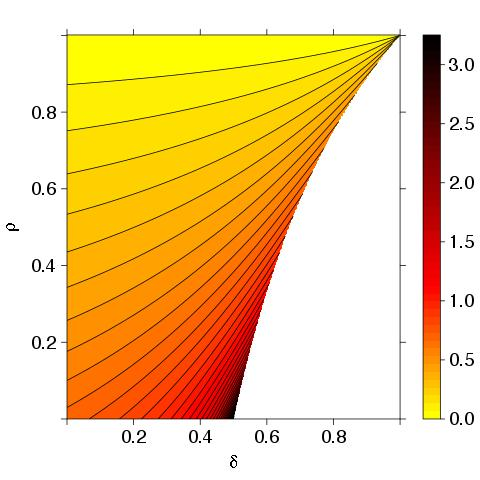
\includegraphics[width=\textwidth]{ExtremeN2}
\caption{N = 2}	
\label{ExtremeN2}
        \end{subfigure}%
        \begin{subfigure}[b]{0.499\textwidth}
                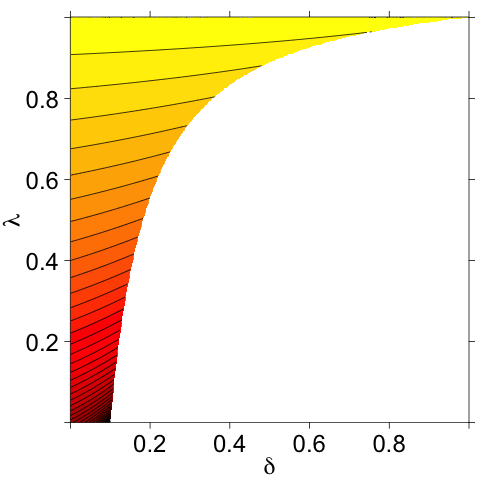
\includegraphics[width=\textwidth]{ExtremeN10}
\caption{N = 10}
\label{ExtremeN10}
        \end{subfigure}
        \caption{ The amount of log-extremizing $\log(\alpha)$ under different combinations of $N$ (the number of experts), $\delta$ (the average amount known by one expert), and $\lambda$ (the average amount shared by any two experts).}
        \label{Levelplots}
\end{figure}
 

This theorem combined with Theorem \ref{positiveProbThm} shows that (\ref{CompoundAggre}) is more often closer to crowd belief than the probit opinion pool is. The amount of extremizing that (\ref{CompoundAggre}) performs for the probit opinion pool is
\begin{align}
%\alpha \bar{X}  &=  \frac{\frac{1}{(N-1)\lambda +1} \sum_{j=1}^N X_j }{\sqrt{T- \frac{N}{(N-1)\lambda +1} }}\\
%\alpha &= \frac{\frac{1}{(N-1)\lambda +1} \sum_{j=1}^N X_j }{\bar{X} \sqrt{T- \frac{N}{(N-1)\lambda +1} }}\\
\alpha &= \frac{\frac{N\sqrt{1-\delta}}{(N-1)\lambda +1}}{\sqrt{1- \frac{N\delta}{(N-1)\lambda +1} }} \label{CompoundAlpha}
% &= \frac{\frac{N}{(N-1)\lambda +1}}{\sqrt{1-\delta  \left( \frac{N}{(N-1)\lambda +1}  \right)}} \\
% &= \frac{\gamma}{\sqrt{1-\delta\gamma}},
% &= \frac{N}{\sqrt{((N-1)\lambda +1)^2 (T- \frac{N}{(N-1)\lambda +1} )}}\\
% &= \frac{N}{\sqrt{((N-1)\lambda +1)^2T- N((N-1)\lambda +1) )}}
\end{align}
%where 
%\begin{align*}
%\gamma &= \frac{N}{(N-1)\lambda +1}\\
%&= \left( \frac{1}{(N-1)\lambda +1} \right) N\\
%\end{align*}
%WHAT IS GAMMA? Given that 
%\begin{align*}
%\gamma \delta &\leq 1\\
%% \frac{N \delta}{(N-1)\lambda +1}  &\leq& 1\\
% \frac{N\delta - 1}{N-1}  &\leq \lambda,
%\end{align*}
%The domain restriction (\ref{rhoDomain}) ensures that the term under the square-root in (\ref{CompoundAlpha}) is always non-negative.  
%Given that the square-root is not defined for negative values,  it must be required that
%\begin{align}
%1- \frac{N\delta}{(N-1)\lambda +1}  &\geq 0 &\Leftrightarrow&& \lambda \geq \frac{N\delta - 1}{N-1} \label{rhoDomain2}
%\end{align}
%Compare this with former domain restriction (\ref{rhoDomain}) and observe that both $N\delta - 1$ and $N - \delta^{-1}$ are negative when $\delta < 1/N$. Given that $N\delta - 1 > N - \delta^{-1}$ only when $\delta < 1/N$, the latter restriction (\ref{rhoDomain2}) is redundant and can be ignored. 
%Given that (\ref{CompoundAlpha}) is increasing in $N$ and $\delta$ but decreasing in $\lambda$, the amount of extremizing can be considered increasing in the total amount of information among the experts.
This is a non-random quantity depends only on three intuitive parameters. Therefore it can be conveniently analyzed graphically. Figure \ref{Levelplots} describes the amount of log-extremizing $\log(\alpha)$ under all plausible combinations of $\lambda$ and $\delta$ under $N = 2$ and $N = 10$ experts. High values have been censored to keep the scale manageable. Even though the patterns in Figure \ref{ExtremeN10}  are very similar to the ones shown earlier in Figure \ref{LevelplotsOracle}, comparing $\alpha$ under $N = 2$ and $N = 10$ leads to new observations. First, holding both $\delta$ and $\lambda$ fixed, the amount of extremizing $\alpha$ increases in $N$. This can be considered as being caused by an increase in the total amount of information among the experts because $\delta'$ is increasing in $N$. Second, in general, having many experts, each with a considerable amount of information, simply leads to unavoidable information overlap. This is illustrated in Figure \ref{Levelplots} where the set of possible values of $\lambda$ decreases very rapidly as $\delta$ increases. Furthermore, moving from Figure \ref{ExtremeN2} to Figure \ref{ExtremeN10} illustrates how the dependence between $\lambda$ and $\delta$ strengthens as $N$ increases. Based on the domain restriction (\ref{rhoDomain}), the value of $\lambda \to 1$ as $N \to \infty$ under any given $\delta$. Therefore in the limit the group of experts is equivalent to a single expert. This restrictive limiting behavior is due to assuming that each pair of experts shares the same amount of information. The compound symmetric information structure, however, is almost fully general when $N = 2$. Therefore assuming compound symmetric information can be appropriate for small numbers of experts but becomes overly restrictive as more experts enter the group. 
%, the probit opinion pool appears to have a similar relationship with  (\ref{CompoundAggre}) and the oracle expert does. 








%\textcolor{red}{This shows that extremizing is not only due to the experts' inability to merge their information.}

 
% Given that this amount increases as a) the amount of information that each individual expert $\delta$ holds increases, and/or b) the amount of shared information $\lambda$ decreases, the more knowledgable and diverse the group of experts is, the more their average probit-forecast should be extremized. The only exception occurs when $\lambda = 1.0$. In this case, all information is public, and the group of experts is as good as a single expert. Therefore, given that a single expert's forecast should not be extremized, $\lambda = 1.0$ always implies $\alpha = 1.0$ regardless of the value of $\delta$. From the top of the graph the extremizing factor increases indefinitely towards the point $\delta = 1/N$ and $\lambda = 0$. At this point the experts' information sets form a partition of the full information. Therefore the experts know all the information. Such a group of experts can re-construct $X_S$ by simply adding up their  information. This is equivalent to deterministic voting: if the sum of the probit-forecasts is above 0, the event $A$ materializes; else it does not. A similar observation has been made under the interpreted forecasts (\cite{hong2009interpreted}). 
%Recall from earlier discussion that the compound symmetric information structure invalidates the possibility of a dominant expert. As (\ref{CompoundAlpha}) does not depend on $\boldsymbol{X}$, the amount of extremizing cannot be driven by highly influential information either. Therefore the amount of extremizing is unaffected by both causes of reverse-extremizing. Consequently, the aggregator (\ref{CompoundAggre}) always extremizes $\bar{P}$.   This is stated more formally in the following Theorem along with the fact that the aggregator (\ref{CompoundAggre}) can leave the convex hull of the individual probabilities. 






\section{Discussion}

% What did we learn from this ?

% 1. In the real world there does not seem to be the two causes of reverse-extremizing. X
% 2. Illustrated that parameters can be estimated X
% 2b. Future work: learning about overlap structures X
% 3. Summarize main observations: 
% (i) extremizing increases as a function of information in the group. X
% (ii) Voting works well under high diversity. 
% 4. Process can be repeated for something else besides extremizing X
% 5. Limitation: Discuss optimality constraint 
% 6. The model checks with intuition. X

% 7. Overall, the procedure resembles voting. Therefore voting can be expected to work well in practice when the voters form a very knowledgable and diverse group of experts.

%\textcolor{red}{discuss how diversity and total information relate to the probit: under probit opinion pool individuals work with their own knowledge, report an estimate that reflects only this information. Therefore the aggregate is as good as the best forecaster is. It cannot extend beyond this to make use of the group's information. }

This paper introduced a concrete model for probability forecasts made by a group of experts. The experts are assumed to make their forecasts based on different subsets of information that ultimately deicides the outcome of the event. The model was used to derive an expression for the best in-principle forecast given the knowledge of $N$ experts. Even though this aggregate, called the crowd belief, may not be accessible in practice, it was used as a theoretical ``gold standard`` for linking extremizing of average aggregates with the information among the experts. The analysis gave two main results. First, the amount of extremizing is increasing in information diversity and the total amount of information among the experts. Second, no matter how information is distributed among the experts, extremizing the probit opinion pool is more likely to beneficial than harmful as long as the experts' forecasts are not all the same. This was a partial motivation for developing an aggregator that always extremizes the average probit-forecast. The partial information aggregator under compound symmetric information was shown to extremize the average probit-forecast as long as the experts' forecasts are not all the same. This aggregator depends only on two intuitive parameters, namely the average amount of information known by an expert and the average amount of information shared between any two experts. Given that these two quantities can be directly estimated from the experts' forecasts, the aggregator can be appropriate for combining forecasts of a one-time event. 

It is interesting to relate our discussion to the many empirical studies conducted by the Good Judgment Project (GJP) (\cite{mellers2014psychological, ungar2012good}). The GJP is a research study that has recruited thousands of forecasters from professional societies, research centers, and alumni associations. These forecasters are given questions about future international political events, such as who would win an election in Russia or the Congo. Individuals then estimate the probability of each event, and update their predictions when they feel the probabilities have changed. The forecasters know that their probability estimates are assessed for accuracy using Brier scores, i.e. the squared distance from the  probability forecast to $1.0$ or $0.0$ depending on whether the event happened or not, respectively (\cite{Brier}). This incentivizes the forecasters to report their true beliefs instead of attempting to game the system (\citet{winkler1968good}). In addition to receiving \$150 for meeting minimum participation requirements that did not depend on prediction accuracy, the forecasters receive status rewards for their performance via leader-boards displaying Brier scores for the top 20 experts. Every year the top 2\% percent of the forecasters are selected to the elite group of ``super-forecasters". The super-forecasters work in groups to make highly accurate predictions on the same events as the rest of the forecasters. 


%The super-forecasters are highly knowledgeable (i.e. they have a high $\delta$) individuals who work in groups (i.e. they have a high $\rho$ and $\lambda$) to make accurate predictions on the same events as the rest of the forecasters. 


Generally extremizing has been found to improve the aggregate predictions (\cite{mellers2014psychological}). The average forecast of a team of super-forecasters, however, often requires very little or no extremizing. This can explained by the partial information model as follows. Given that the  super-forecasters are highly knowledgeable (i.e. they have a high $\delta$) individuals who work in groups (i.e. they have a high $\rho$ and $\lambda$), they are situated in Figures \ref{LevelplotsOracle} and \ref{Levelplots} around the upper-right corners where almost no extremizing is required. All forecasters were also asked to self-assess their level of expertise (on a $1$-to-$5$ scale with $1$ = Not At All Expert and $5$ = Extremely Expert) on the events for which they provided forecasts. Given that expertise is largely defined by the forecaster's personal knowledge, the value of $\delta$ can be considered positively associated with the self-assessed expertise. Marginally, this implies a positive relationship between the level of expertise and amount of extremizing. \cite{satopaa}, however, suggest that the amount of extremizing is negatively associated with self-assessed expertise, i.e. lower expertise requires more extremizing. This can be explained by two observations. First, the average number of forecasters $N$ per expertise group across the $69$ international events considered in \cite{satopaa} were around $68.3$, $84.9$, $61.6$, $17.5$, and $3.4$ (from the lowest to the highest level of expertise). Second, as illustrated by Figure \ref{Levelplots}, the low experts had a chance of being highly diverse while the high experts were likely to experience considerable information overlap. These observations suggest that the low-expertise groups required more extremizing because they held more information in total than the high-expertise groups.


The partial information model offers many future research directions. For instance, new probability aggregators can be developed by finding different ways  to estimate the information overlap among experts. Unfortunately, without any additional information besides the probability forecasts, it may not be possible to estimate the information structure accurately in full generality. Therefore the structure must be constrained in some manner. For instance, Appendix A provides explicit estimation instructions under the compound symmetric information structure. This structure, however, has poor limiting behavior. Therefore it will be necessary to develop a class of information structures that is  both estimable and more realistic for large numbers of experts.  A different alternative is to construct a prior distribution for the information structure, update this prior to a posterior distribution via the multivariate Gaussian likelihood function, and then marginalize the information structure with respect to its posterior distribution.  

 
 Other future directions could  remove some of the model limitations. For instance, assuming that the experts produce optimal probability forecasts given their private information sets may not be reasonable. The experts can believe in false information, hide their true beliefs, or be biased for many other reasons. This could be expressed in the model by introducing an error term that is added to the optimal forecasts before being assigned to the experts. Such an extension was not considered in this paper for the sake of providing a clean introduction to the partial information model together with a clear illustration of our main results on  probability extremizing. 
 
  \appendix 
\section*{Appendix A: Technical Details}
\label{appendix}

\subsection*{A.1  Proofs}
%\textit{Proof of Theorem \ref{positiveThmVote}.} Let $\boldsymbol{d} = \frac{1}{N}\left((1-\delta_1)^{-1/2}, (1-\delta_2)^{-1/2}, \dots, (1-\delta_N)^{-1/2}\right)'$. Assume without loss of generality that $\bar{P} > 0$. Then the average probit forecast is extremized if
%\begin{align}
% \bar{P}&\leq  \frac{\sum_{j=1}^N X_{I_j}}{\sqrt{1 - \sum_{j=1}^N \delta_j}} &\Leftrightarrow&& 0 \leq  \left\{  \left(1 - \sum_{j=1}^N \delta_j \right)^{-1/2} \boldsymbol{1}_N - \boldsymbol{d}' \right\} \boldsymbol{X} \label{votingproof}
%\end{align}
% As $N (1-\delta_j)^{1/2} \geq \left(1 - \sum_{j=1}^N \delta_j \right)^{1/2}$ for all $j = 1, \dots, N$, all the elements of $$\left(1 - \sum_{j=1}^N \delta_j \right)^{-1/2} \boldsymbol{1}_N - \boldsymbol{d}' $$ are non-negative. Therefore the right hand side of (\ref{votingproof}) is always non-negative. \qed
% \\
% \\
%\noindent

\textit{Proof of Theorem \ref{positiveProbThm}.}
\begin{align*}
x_0 &= \kappa \frac{\sigma_1}{\sigma_2} \\
 &= \frac{ \sum_{j=1}^N \frac{\delta_j}{\sqrt{1-\delta_j}}}{\sqrt{\delta'  \left( \sum_{j=1}^N \frac{\delta_j}{1-\delta_j} + 2 \sum_{i,j: i<j} \frac{\rho_{ij}}{\sqrt{(1-\delta_j)(1-\delta_i)}}\right)}} \sqrt{\frac{\frac{\delta'}{1-\delta'}}{\frac{1}{N^2} \left( \sum_{j=1}^N \frac{\delta_j}{1-\delta_j} + 2 \sum_{i,j: i<j} \frac{\rho_{ij}}{\sqrt{(1-\delta_j)(1-\delta_i)}}\right) }}\\
%&=  \frac{N \sum_{j=1}^N \frac{\delta_j}{\sqrt{1-\delta_j}}}{\sqrt{ \left( \sum_{j=1}^N \frac{\delta_j}{1-\delta_j} + 2 \sum_{i,j: i<j} \frac{\rho_{ij}}{\sqrt{(1-\delta_j)(1-\delta_i)}}\right)}} \sqrt{\frac{\frac{1}{1-\delta'}}{ \left( \sum_{j=1}^N \frac{\delta_j}{1-\delta_j} + 2 \sum_{i,j: i<j} \frac{\rho_{ij}}{\sqrt{(1-\delta_j)(1-\delta_i)}}\right) }}\\
%&=  \frac{N \sum_{j=1}^N \frac{\delta_j}{\sqrt{1-\delta_j}}}{ \sum_{j=1}^N \frac{\delta_j}{1-\delta_j} + 2 \sum_{i,j: i<j} \frac{\rho_{ij}}{\sqrt{(1-\delta_j)(1-\delta_i)}}} \sqrt{\frac{1}{1-\delta'}}\\
&=  \frac{N \sum_{j=1}^N \frac{\delta_j}{\sqrt{(1-\delta_j)(1-\delta')}}}{ \sum_{j=1}^N \frac{\delta_j}{1-\delta_j} + 2 \sum_{i,j: i<j} \frac{\rho_{ij}}{\sqrt{(1-\delta_j)(1-\delta_i)}}}
%&\geq  1
%&=  \frac{\frac{1}{N} \sum_{j=1}^N \frac{\delta_j}{\sqrt{(1-\delta_j)(1-\delta')}}}{\frac{1}{N^2} \left( \sum_{j=1}^N \frac{\delta_j}{1-\delta_j} + 2 \sum_{i,j: i<j} \frac{\rho_{ij}}{\sqrt{(1-\delta_j)(1-\delta_i)}} \right)}\\
\end{align*}
Given that all the remaining terms are positive, the location parameter $x_0$ is also positive. Next compare the $N$ terms with a given subindex $j$ in the numerator with the corresponding terms in the denominator. As $\delta' \geq \delta_j$ and $\delta' \geq \rho_{ij}$, then 
\begin{align}
\frac{\delta_j}{1-\delta_j} = \frac{\delta_j}{\sqrt{(1-\delta_j)(1-\delta_j)}} &\leq \frac{\delta_j}{\sqrt{(1-\delta_j)(1-\delta')}} \label{ProofIneq1}\\
 \frac{\rho_{ij}}{\sqrt{(1-\delta_j)(1-\delta_i)}} &\leq \frac{\delta_j}{\sqrt{(1-\delta_j)(1-\delta')}} \label{ProofIneq2}
\end{align}
Therefore 
\begin{align*}
N \sum_{j=1}^N \frac{\delta_j}{\sqrt{(1-\delta_j)(1-\delta')}} \geq \sum_{j=1}^N \frac{\delta_j}{1-\delta_j} + 2 \sum_{i,j: i<j} \frac{\rho_{ij}}{\sqrt{(1-\delta_j)(1-\delta_i)}},
\end{align*}
which gives that $x_0 \geq 1$. Therefore, as the Cauchy distribution is symmetric around $x_0$, it must be the case that $\P(\alpha \geq 1 | \Sigma_{22}) \geq 0.5$. Based on (\ref{ProofIneq1}) and (\ref{ProofIneq2}), the location $x_0 = 1$ only when all the experts know the same information, i.e. when $\delta_j = \delta'$ for all $j = 1, \dots, N$. Under this particular setting, the amount of extremizing $\alpha$ is non-random and always equal to $1.0$. Therefore $\P(\alpha \geq 1 | \Sigma_{22}) = 1.0$.  Any deviation from this particular information structure makes $\alpha$ stochastic, $x_0 > 1$, and hence $\P(\alpha \geq 1 | \Sigma_{22}) > 0.5$. If the expert's information sets partition the full information, the sum of their probits is always on the correct side of $0.0$. At the same time the oracle deterministically outputs the correct outcome. Consequently, $\alpha = +\infty$ and $\P(\alpha \geq 1 | \Sigma_{22}) = 1$. Thus $\P(\alpha > 1 | \Sigma_{22}) \in (0.5, 1.0]$ when $\delta_j \neq \delta'$ for some $j = 1, \dots, N$. \qed
\\
\\
\noindent
\textit{Proof of Theorem \ref{positiveThm}.} (a) For a given $\delta$, the amount of extremizing $\alpha$ is minimized when $(N-1)\lambda +1$ is maximized. This happens as $\lambda \uparrow 1$. Plugging this into (\ref{CompoundAlpha}) gives
\begin{align*}
\alpha &= \frac{\frac{N\sqrt{1-\delta}}{(N-1)\lambda +1}}{\sqrt{1- \frac{N\delta}{(N-1)\lambda +1} }}  \uparrow \frac{\sqrt{1-\delta}}{\sqrt{1-\delta }} = 1
\end{align*}
(b) Assume without loss of generality that $\bar{P} > 0$. If $\max(\left\{p_1, p_2, \dots, p_N \right\}) < 1.0$, then  setting $\delta = 1/N$ and $\lambda = 0.0$ gives an aggregate probability $\P\left(X_S > 0 | \boldsymbol{X}\right) = 1.0$ that is outside the convex hull of the individual probabilities.
\qed

\subsection*{A.2 Estimation of $\delta$ and $\lambda$}


The values of $\delta$ and $\lambda$ can be estimated via the maximum likelihood method. To make this more explicit, observe that the Jacobian for the map $\boldsymbol{P} \to \Phi\left(\boldsymbol{P}\right) = (\Phi(P_1), \Phi(P_2), \dots, \Phi(P_N))'$ is
\begin{eqnarray*}
J(\boldsymbol{P}) &=& (2\pi)^{-N/2} \exp \left( - \frac{\boldsymbol{P}' \boldsymbol{P}}{2}   \right) 
\end{eqnarray*}
%
%$\boldsymbol{P} \sim \mathcal{N}_N\left(\boldsymbol{0}, \Sigma_{22} (1-\delta)^{-1}\right)$ and that
Let $J_{N \times N}$ represent a $N\times N$ matrix of ones. If $h(\boldsymbol{P})$ denotes the multivariate Gaussian density of $\boldsymbol{P} \sim \mathcal{N}_N\left(\boldsymbol{0}, \Sigma_{22} (1-\delta)^{-1}\right)$,
%by the Inverse Function Theorem 
the density for  $\boldsymbol{p} = (p_1, p_2, \dots, p_N)'$ becomes
\begin{eqnarray*}
 f\left(\boldsymbol{p} | \delta, \lambda \right) &=& h(\boldsymbol{P}) J(\boldsymbol{P})^{-1} \bigg|_{\boldsymbol{P} = \Phi^{-1}(\boldsymbol{p})}\\
%&=& \frac{(1-\delta)^{N/2}}{\sqrt{ |\Sigma_{22}|}} \exp\left( -\frac{1}{2} \boldsymbol{P}' (1-\delta)\Sigma_{22}^{-1} \boldsymbol{P} + \frac{\boldsymbol{P}' \boldsymbol{P}}{2}   \right)\\
&=& \frac{(1-\delta)^{N/2}}{\sqrt{ \left|\Sigma_{22}\right|}} \exp\left[ -\frac{1}{2} \Phi^{-1}(\boldsymbol{p})' \left\{ (1-\delta) \Sigma_{22}^{-1} - I_N \right\} \Phi^{-1}(\boldsymbol{p})  \right],
\end{eqnarray*}
%where $\Phi^{-1}(\boldsymbol{p}) =  (\Phi^{-1}(p_1), \Phi^{-1}(p_2), \dots, \Phi^{-1}(p_N))$. 
%Given that $\Sigma_{22}$ can be written in the form  $\Sigma_{22} = I_N (\delta-\lambda\delta) + J_{N \times N} \lambda\delta$
where
%The determinant and inverse of $\Sigma_{22}$ are
\begin{align}
\left| \Sigma_{22}\right| &= (\delta(1- \lambda))^N \left(1+\frac{N \lambda}{1 - \lambda} \right) \nonumber\\
\Sigma_{22}^{-1} &= I_N \left(\frac{1}{\delta-\lambda\delta} \right) - J_{N \times N} \frac{\lambda}{(1-\lambda)\delta\{1+(N-1) \lambda\}} \label{inverse}
\end{align}
See \cite{rao2009linear} and the supplementary material of \cite{dobbin2005sample} for the derivations of the determinant and inverse of $\Sigma_{22}$, respectively. The maximum likelihood estimates of $\delta$ and $\lambda$ are then obtained from
\begin{align*}
\left(\hat{\delta}, \hat{\lambda}\right) =& \argmax_{\lambda, \delta} \log  f\left(\boldsymbol{p}| \delta, \lambda \right),\\
& \text{s.t. } \nonumber \delta \in [0,1] \text{ and } \lambda \in \left[  \max \left\{ \frac{N-\delta^{-1}}{N-1}, 0\right\}, 1 \right)
\end{align*}
%\textcolor{red}{check if this is a convex program}
Given that this cannot be solved analytically, numerical methods such as a simple grid-search must be used to find $\hat{\delta}$ and $\hat{\lambda}$. 

% 

\bibliographystyle{Chicago}
%\bibliographystyle{plainnat}
\bibliography{biblio}		% expects file "myrefs.bib"



\end{document}
